
\documentclass[natbib,referee]{svjour3}

\smartqed  % flush right qed marks, e.g. at end of proof


% PACKAGES
% ------------------------------------------------------------------------------

\usepackage{simplemargins}
\usepackage{textcomp}
\usepackage{amsbsy}
\usepackage[dvipsnames]{xcolor}

\usepackage{graphicx}
\usepackage[pdftex,bookmarks=false]{hyperref}
\usepackage{float}
 \usepackage{multirow}

% LINKS
% ------------------------------------------------------------------------------

\hypersetup{
    pdfpagelayout=OneColumn,
    colorlinks = true,
    urlcolor   = blue,
    citecolor  = blue,
    linkcolor  = blue
}
\urlstyle{same}


% ADDITIONAL COMMANDS
% ------------------------------------------------------------------------------

\newcommand{\myrevision}[1]{\textcolor{Black}{#1}}
\settopmargin{1.2in}
\setleftmargin{.9in}
\setrightmargin{1in}
\setbottommargin{.2in}


% JOURNAL NAME
% ------------------------------------------------------------------------------

\journalname{Not Decided}


% MAIN DOCUMENT STARTS
% ==============================================================================


\newcommand{\vsmin}{$V_{S_{\min}}$}
\newcommand{\vsmineq}[1]{$V_{S_{\min}}=#1$~m/s}
\newcommand{\vsthirty}{$V_{S30}$}
\newcommand{\vs}{$V_{S}$}
\newcommand{\vseq}[1]{$V_{S}=#1$~m/s}

\newcommand{\vp}{$V_{P}$}
\newcommand{\vpeq}[1]{$V_{P}=#1$~m/s}

\newcommand{\qp}{$Q_{P}$}
\newcommand{\qs}{$Q_{S}$}
\newcommand{\qk}{$Q_{K}$}
\newcommand{\qsvs}{$Q_{S}-V_{S}$}
\newcommand{\qpqs}{$Q_{P}-Q_{S}$}
\newcommand{\qsoqp}{$Q_{S}/Q_{p}$}

\newcommand{\feq}[1]{$f=#1$~Hz}
\newcommand{\fleq}[1]{$f\leq#1$~Hz}
\newcommand{\fgeq}[1]{$f\geq#1$~Hz}
\newcommand{\fmax}{$f_{_{\max}}$}
\newcommand{\fmaxeq}[1]{$f_{_{\max}}=#1$~Hz}

\newcommand{\eqmag}[1]{$M_{#1}$}

\newcommand{\adomain}[3]{#1~#3 $\times$ #2~#3}
\newcommand{\vdomain}[4]{#1~#4 $\times$ #2~#4 $\times$ #3~#4}

\begin{document}


% TITLE
% ------------------------------------------------------------------------------

\title{A Surrogate-based Optimization Approach for Calibration of Attenuation Models (\qsvs{} Relationships) Used in Physics-Based Ground-Motion Earthquake Simulation}
\titlerunning{\qsvs{} Relationships}


% AUTHORS
% ------------------------------------------------------------------------------

\author{%
    Naeem Khoshnevis \and 
    Ricardo Taborda
}

% \authorrunning{N.~Khosh} % if too long for running head

\institute{
    N. Khoshnevis
       \at
        Center for Earthquake Research and Information\\
        The University of Memphis, Memphis, TN 38152, U.S.A.\\
        \email{nkhshnvs@memphis.edu}\\
    R. Taborda 
        \at
        Center for Earthquake Research and Information\\
        and Department of Civil Engineering
        The University of Memphis, Memphis, TN 38152, U.S.A.
}

\date{Received: date / Accepted: date}

\maketitle

\begin{abstract}
    %
We present a customized solution approach to study attenuation models through combining machine learning, ground motion simulation, and optimization methods. The accurate solution of wave propagation problems requires the appropriate representation of energy losses due to internal friction in geomaterials. These losses are important because their mischaracterization may lead to the over- or under-estimation of the amplification and duration of seismic waves in regions with high dissipative properties. Recent studies show that synthetics from physics-based simulations tend to attenuate with distance at different rates than observations, thus suggesting that current approaches to modeling attenuation need to be revised. In physic-based ground-motion simulation, the attenuation of seismic waves is typically treated by means of viscoelastic models. Internally, the properties used for these models are set based on the material's quality factor Q. The value of Q for shear waves, Qs, for instance, is usually defined based on rules that depend on the value of the shear wave velocity, Vs.  Typical Qs-Vs relationships are (piecewise) linear or polynomial functions. Several Qs-Vs relationships exist in the literature. There is, however, no consensus about the most appropriate one. In addition, other studies suggest that these relationships vary for P waves, and are dependent of depth. 
We propose new methodology based on  combining machine learning (artificial neural network) techniques and optimization methods to narrow and customize the search domain for each individual stations in studying the Q factor parameters in physics-based ground motion simulation. We successfully tested the proposed method in homogeneous, layered, and actual heterogenous domains. The proposed method shows how emerging computational resources and machine learning techniques can improve scientific research. Working with observational data, due to noise, potential rotation of stations during earthquake, mistakes in preprocessing data and many more other factors, in many cases, make the search process very difficult. The proposed method, gives the idea of actual search area, before start woking with observations. We tested the proposed model based on $Mw ~5.4$ 2008 Chino Hills earthquake's recorded data and present the optimal Q model. 




    \keywords{Anelastic attenuation \and 
3D ground motion simulation \and
Machine Learning \and
Customized solution\and 
Los Angeles Basin 
}
\end{abstract}



\section{Introduction}

The advances in ground motion simulation techniques and high performance computational resources, and comprehensive studies of velocity models make regional scale ground motion simulations more accurate and possible for higher frequencies ($fmax < 5 Hz$). Complicated source models and  geological features (i.e., heterogeneous velocity models) introduce a broad variation in parameters for each seismic station. Due to mentioned complexities, for one particular earthquake, based on current knowledge about the domain and seismic behavior of them, different stations can be helpful in variable level in studying ground motion simulation parameters. It is a common practice to consider all stations results and compute a average the parameters as a finial result. However, with the complexity involved in the model and in reality,  all stations for different earthquakes are not contributing the same information at the same level. Therefore, a comprehensive study should be considered to understand whether each station due to its distance and azimuth from source, as well as its site characterization have a potential to provide useful information about the research parameter. In other words, we need to take customized approaches toward each station. Therefore, before comparing the results with observation we need to setup a system to understand what information we can extract from the model and consequently from each station. Application of this idea is possible due to mentioned advances in physics-based ground motion simulation technics, however, due to need for considerable computational resources and significant time for simulations, sensitivity and optimization analyses are barely considered for these solutions. Machine learning technics, specifically artificial neural networks, are very trustable tools to be trained as a complicated nonlinear functions and predict accurate results in a short time, providing enough training data. This idea can have a broad application in seismology and physics-based ground motion simulation.  In this paper, however,  we focus on the application of the proposed method on studying the seismic quality factor (Q factor) parameters for physics-based ground motion simulation. Although customized solution for each seismic station is not a common practice in seismology, however, customized solutions have been studied and discussed in other fields of science. Specifically, personalized medicine research is a hot topic in health care studies \citep{weiss2012machine,jin2009hearttogo,katsios2010individual,hamburg2010path,offit2011personalized}. \\
In this paper we study the application of a customized solution idea in seismic attenuation model parameters. The amplitude of seismic waves decreases as the distance from source increases. In the absence of large deformations (nonlinearities), this is due to: Geometric spreading, intrinsic attenuation, and scattering. Geometric spreading and scattering (due to heterogenous velocity model) are inherently considered in 3D ground motion simulation. Intrinsic attenuation, on the other hand,  happens due to irreversible changes in the crystal defect structures of the medium. These media are called anelastic and the configuration of material particles is to some extended dependent on the history of applied stress \citep{aki2002quantitative}. Intrinsic attenuation or internal friction is studied by means of quality factor (Q) which is inversely related to the strength of the attenuation. In seismology, anelastic damping is studied from different perspective for different application.   From the definition of Q factor (fractional energy loss per cycle) it is concluded that the rate of attenuation increases with frequency. Therefore, Q is considered as frequency depended \citep[e.g., see][ and references therein.]{adams1998seismic, withers2013deterministic, mousavi2014average, sedaghati2015estimation, nazemi2017attenuation}. For high frequency Q factor,  \citet{hauksson2006attenuation} showed that the Qp (anelastic damping related to P-wave) and Qs can be different on a regional scale due to  local impedance contrasts, chemical composition, crack structure, grain boundary movement, crustal fluids, and, to a lesser extent, temperature variations within the brittle seismogenic crust. However, many studies showed that the frequency dependency of Q is significant at higher frequencies $( f > 1 Hz)$. In this paper, we are interested in better constraining the parameters of models used to�represent the effects of intrinsic attenuation, that is, the quality factors Qs and Qp, and in particular, the relationships used to correlate Qs with Vs in deterministic ground motion simulation. Given the wavelengths and minimum velocities considered in earthquake simulation in the past, attenuation models have been considered to be frequency independent and the dependence of the Qs-Vs relationships with depth has been ignored. The sensitivity of the ground motion to the relationships used to define the quality factors Qs and Qp based on the shear wave velocity Vs as the primary variable is studied and confirmed. \\
Advances in simulation algorithms and methods, and the increasing capability of parallel applications have made it possible to solve seismic wave propagation problems in large regions with highly heterogeneous media at levels of resolution not thought feasible before. A crucial component of these simulations is the accurate representation of the crustal structure using three-dimensional (3D) material models. This entails the definition of the density, the seismic velocities, and the attenuation properties at arbitrary points over large regions. The accurate solution of the wave propagation problem itself also requires the appropriate representation of the energy losses that occur due to internal friction in geomaterials. These losses are important because their omission may lead to the overestimation of the amplification and duration of seismic waves in regions with high dissipative properties.\\
In physic-based earthquake ground-motion simulation, the attenuation of seismic waves is typically treated by means of viscoelastic models \citep[e.g.,][]{day2001memory, graves2003stability, kaser2007arbitrary, Bielak2011}. These models are made of mechanisms that employ numerical techniques to account for the dissipative and transient characteristics of the ground motion. Internally, the properties of a given attenuation model are set based on the material's quality factor, Q. Community velocity models (CVMs) used in simulations do not generally provide values of Q. Instead, the most common approach is to define the quality factors associated with P- and S-waves, Qp and Qs, based on the values of the seismic velocities Vp and Vs obtained from any particular CVM.\\
The value of Qs, for instance, is usually defined based on rules that depend on the value of Vs. Typical forms of $Qs-Vs$ relationships are (piecewise) linear or polynomial functions \citep[e.g.,][]{brocher2008compressional, brocher2005compressional,olsen2003estimation, graves2008seismic,taborda2013ground}. On the other hand, the value of Qp is usually defined in terms of Qs, and, in some cases, also on the velocity contrast Vp/Vs. Table. ~\ref{tab:QsVstable} shows a collection of different Qs-Vs and Qp-Qs relationships used in simulations and other related studies, including the earthquake or scenario event for which they were employed, and the simulation's minimum shear wave velocity (Vsmin) and maximum frequency (fmax).\\
% Please add the following required packages to your document preamble:
% \usepackage{multirow}
\begin{table}[]
	\centering
	\caption{Examples of \qsvs{} and \qpqs{} relationships used in past physics-base simulations}
	\label{tab:QsVstable}
	\renewcommand{\arraystretch}{0.75}
	\resizebox{\textwidth}{!}{%
		\begin{tabular}{lccccccc}
			\textbf{Publication}                                                        		    & \textbf{Simulation}                                       &  \textbf{\vsmin{}}             & \textbf{\fmax{}}                          & \multicolumn{3}{c}{\textbf{\qs{}=g(\vs{})}}                     &\textbf{\qp{}=h(\qs{})}                                 \\ 
			                                                                                       		    &                                                                     &  \textbf{(m/s)    }             & \textbf{(Hz)}                                 & \multicolumn{3}{c}{\textbf{($V_{S}$ in km/s, depth $z$ in km)}}         &                               \\ \hline
			\citet{Olsen_2003_BSSA}                                             		    & 1994 Northridge                                          & \multirow{2}{*}{500}        & \multirow{2}{*}{0.5}                    & 20\vs{}                                                             &   & \vs{}$< 1.5$                           & \multirow{2}{*}{1.5\qs{}} \\ 
			\citet{Olsen_2008_BSSA}                                              		    & TeraShake$$                                               &                                        &                                                   & 100\vs{}                                                           &   & \vs{} $\geq 1.5$                       &                            \\\hline
			\citet{Olsen_2009_GRL}                                               		    & ShakeOut                                                    & \multirow{3}{*}{500}        & \multirow{3}{*}{0.5}                    & \multicolumn{3}{c}{\multirow{4}{*}{50\vs{}}}     & \multirow{4}{*}{2\qs{}}                             \\
			\citet{Bielak_2010_GJI}$^{FD}$                                    		    &  ShakeOut                                                   &                                        &                                                   & \multicolumn{3}{c}{}                                          &                                                 \\
			\citet{Graves_2011_PAG}                                              		    & CyberShake                                                &                                         &                                                  & \multicolumn{3}{c}{}                                          &                                                 \\ \cline{3-4}
			\citet{Cui_2010_Proc}                                                   		    & M8                                                               & 400                                  & 2.0                                            & \multicolumn{3}{c}{}                                          &                                                 \\ \hline
			\multirow{2}{*}{\citet{Komatitsch_2004_BSSA}}             		    & 2001 Hollywood                                          & \multirow{2}{*}{670}         & \multirow{2}{*}{0.5}                   & 90                                 &   & Sediments                              & \multirow{2}{*}{$\infty$}  \\
			                                                                                        		    & 2002 Yorba Linda                                        &                                         &                                                  & $\infty$                           &   & Bedrock                                &                            \\ \hline
			\citet{Taborda_2006}$^\mathsection$                              		    & TeraShake                                                   & 300                                  & 1.0                                            & \multicolumn{3}{c}{\multirow{3}{*}{50\vs{}}}                                                                                  &                                                                 \\
			\citet{Taborda_2007} $^\mathsection$                            	            & ShakeOut                                                    & 200                                  & 1.0                                             & \multicolumn{3}{c}{}                                                                                                                    &                                                                  \\
			\citet{Bielak_2010_GJI}$^{FE,}$$^\mathsection$                            & ShakeOut                                                   & 500                                   & 0.5                                            & \multicolumn{3}{c}{}                                                                                                                    &                                                                 \\ \hline
			\citet{Graves_2008_BSSA}                                    		             & 2001 Big Bear                                            & 250                                   & 1.0                                            & \multicolumn{3}{c}{60\vs{}}                                                                                                           &                                                 \\ \cline{5-7}
			\multirow{3}{*}{\citet{Aagaard_2008_BSSA}}            			     & \multirow{3}{*}{1989 Loma Prieta}             & \multirow{3}{*}{330-760}   & \multirow{3}{*}{0.5-1.0}             & $50V_{S}$         &   & $V_{S}< 0.9$                           & \multirow{6}{*}{$2$\qs{}}  \\
			                                                                                    		  	     &                                                                    &                                         &                                                   & $60 V_{S}^{1.5}$                   &   & $0.9 \leq V_{S}<3.4$                   &                            \\
			                                                                                       		     &                                                                    &                                         &                                                  & $500$                              &   & $3.4 \geq V_{S}$                       &                            \\ \cline{5-7}
			\multirow{3}{*}{\citet{Brocher_2008_BSSA}$^\mathparagraph$}     &                                                                     &                                        &                                                   & 13                                 &   & $V_{S}<0.3$                            &                            \\
			                                                            					    &                                                                     &                                         &                                                   & $-16+104.13V_{S}$                  &   & \multirow{2}{*}{$0.3\leq V_{S} < 5.0$} &                            \\
			                                                            					    &                                                                     &                                         &                                                   & $-25.225{V_{S}}^2+8.2184{V_{S}}^3$ &   &                                        &                            \\ \hline
			\citet{Chaljub_2010_BSSA}$^\dagger$                                           & 2003 Lancey, and                                        & \multirow{2}{*}{300}        & \multirow{2}{*}{2.0}                     & 50                                 &   & $z<1$                                  & $3/4(V_{P}/V_{S})^2Q_{S}$  \\
			                                                            				            & Event S1                                                      &                                        &                                                    & $\infty$                           &   & $z\geq1$                               & $\infty$                   \\ \hline
			\citet{Taborda_2013_BSSA}                                    			    & \multirow{2}{*}{2008 Chino Hills}                 & \multirow{2}{*}{200}        & \multirow{2}{*}{4.0}                     & \multicolumn{3}{c}{\multirow{3}{*}{\begin{tabular}[c]{@{}c@{}}$10.5 - 16V_{S} + 153 V_{S}^2-103V_{S}^3$\\ $+ 34.7V_{S}^4-5.29*V_{S}^5+0.31V_{S}^6$\end{tabular}}} & \multirow{3}{*}{$3/4(V_{P}/V_{S})^2Q_{S}$} \\
			\citet{Taborda_2014_BSSA}                                    			    &                                                                     &                                        &                                                    & \multicolumn{3}{c}{}                                                                                                                        &                                                 \\ \cline{1-4}
			\citet{Taborda_2016_GJI}                                                                & 30 earthquakes                                           & 200                                  & 1.0                                              & \multicolumn{3}{c}{}                                                                                                                        &                                                 \\ \hline
			\citet{Withers_2015_BSSA}$^\ddagger$                                         & 2008 Chino Hills                                         & 200                                  & 4.0                                               & \multicolumn{3}{c}{$100V_{S}$}                                                                                                       & $2$\qs{}                                              \\ \hline
			\multicolumn{4}{l}{$*$ Denotes scenario events}                                                                                & \multicolumn{4}{l}{$\dagger$ Simulations for Grenoble Valley, France}                                                                                                                                                                                                                   \\
			\multicolumn{4}{l}{$\mathsection$ Rayleigh damping instead of a visco-elastic model}                     & \multicolumn{4}{l}{$^{FE}$ Finite-element simulation results therein}                                                                                                                                                                                                                 \\
			\multicolumn{4}{l}{$\mathparagraph$ Empirical relations (no simulation) for Northern California}     & \multicolumn{4}{l}{$^{FD}$ Finite-difference simulation results therein}            \\
			\multicolumn{4}{l}{$\ddagger$ Frequency independent part of $Q$}                                                  & \multicolumn{4}{l}{}                                                                                                                                                                                                     
		\end{tabular}}
\end{table}
As it can be seen, there is no consensus on the most appropriate set of relationships between seismic velocities and quality factors. The relationship used by \citet{taborda2013ground} was introduced as an attempt to capture some of the main features of other $Qs-Vs$ rules. 
It is known that the relationships between Qs and Vs, and between Qp and Qs can be depth dependent (see, for instance, \citet{olsen2003estimation}, and the references therein) although Qs remains strongly correlated with Vs.  \citet{hauksson2006attenuation} also show that while Qs and Qp increase rapidly with depth in consistency with the crustal structure, but argue that the ratios between Qs and Qp vary with depth and are different within and outside the major basins in southern California. They obtained values of $Qs/Qp > 1$ for most of the region, but found a few limited areas, mostly outside the major sedimentary basins, where $Qs/Qp < 1$. Jordan and Song (2013) concluded that, in general, $Qs \geq Qp$, with $Qs \approx Qp$ near the surface $(z < 5 km)$ but $Qs > Qp$ at depth; and indicated that Qs seems to be in better agreement with the rule $Qs = 50Vs$ at depth but not near the surface, where Qs is not linearly related to Vs. However, most of the simulations done recently (as seen in Table.~\ref{tab:QsVstable}) correspond to numerical models with maximum frequencies, $fmax \leq 1-2 Hz$, and minimum shear wave velocities, $Vsmin \geq 400 m/s$, where one can still assume Q to be frequency independent. Moving forward, it is essential to gather information that allow us to build a consensus about the appropriate choice of Q in simulations. Ideally, this should be done with a rigorous inversion process. This, however, may take a significant amount of time and resources due to the complexity of the problem. \\
Hence fore, In this study we define a Vs dependent quality factor and through using machine learning and optimization process we propose a new approach to study the accurate parameters for physics based ground motion simulation. The method represent significant improvement in narrowing and customizing the search domain and it can be used for more earthquakes, higher frequencies, and different frequency bands. \\ 
In summary, we use genetic algorithm (GA) as an optimization tool to match the synthetic and observation data. However, before comparing with observation and extracting relevant data, for each station we test the model with a known (however, very close to the mean of observation) attenuation parameters. Based on the test scenarios, we understand which range of shear wave velocity of the station has a potential to provide accurate results. Based on the mentioned test, we extract relevant data from the optimization process results.  We test the proposed method on $Mw~5.4$ 2008 Chino Hills earthquake with minimum shear wave velocity of 350 m/s and maximum frequency of 1 Hz. Since the forward simulation on a regional scale requires considerable computational resources and time, conducting this study with actual simulator is practically impossible. Therefore, we generate a pseudo-simulators using neural networks where it can generate the signal parameters with acceptable accuracies in fraction of seconds on one processor instead of using tens of computational nodes to compute them. Our study shows in addition of using peak ground velocity, response spectra, peak ground acceleration, and area under the signal envelop can improve the optimization process functionality and narrow the solution search domain.  It is worth mentioning that the  method is used only for one earthquake in Los Angles basin, using more earthquakes will definitely improve and refine the results, however, the method presented here is a good guideline to plan for numerous earthquake with higher frequency studies. 



















\section{Methodology}

We use a sequence of optimization processes based on observation and synthetic data to find the most appropriate \qsvs{} relationship parameters. The proposed process makes it possible to locate the most accurate shear wave velocity range or effective shear wave velocity range to study \qsvs{} relationship for each seismic station. We use the term of effective shear wave velocity range for the range of \vs{} that a traveling wave has been highly influenced from while propagating in the domain, or based on recorded data and optimization process we can extract $Q$ values for that range of \vs{}. The \qsvs{} relationship is defined as a function of shear wave velocity.  A genetic algorithm (GA) is used to search for the best parameters of this relationship.  In simple words, it efficiently searches for those parameters that result in close to target values. Target values can be acquired from synthetic ground motion simulations or actual observations. GA uses a function, which is known as a cost function, to evaluate the proposed parameters. If it provides good results, it keeps them if not it searches for other parameters unless it finds the best solution or meets the termination criteria. The cost function evaluation is based on signals comparison. It is not possible to compare two signals wiggle by wiggle at higher frequencies (\fmaxeq{0.5}). Therefore, the cost function compares some metrics of signals instead of the whole waveforms.  The synthetic signal is generated based on proposed parameters by GA at iteration. Extracting these metrics, for each set of new parameters, requires running a regional scale ground motion simulation. These runs are computationally expensive and time-consuming. To make this process practical under a reasonable time and computational budget, based on many simulation data, we develop surrogates (or meta-models).  The surrogates are artificial neural networks (ANNs) that are trained to accurately estimate the signal metrics based on \qsvs{} relationship input parameters. Fig.~\ref{fig:Figure_1} shows the method's workflow. The workflow includes four main tasks:
\begin{itemize}
        \item \qsvs{} relationships and ground motion simulations 
	\item Preprocessing signals and extracting signals metrics,
	\item Developing surrogates, 
	\item Running the optimization process to search for the best input parameters, and
	\item Locating the effective shear-wave velocity range and choosing data.  
\end{itemize}

 \begin{figure}[ht]
    \centering
    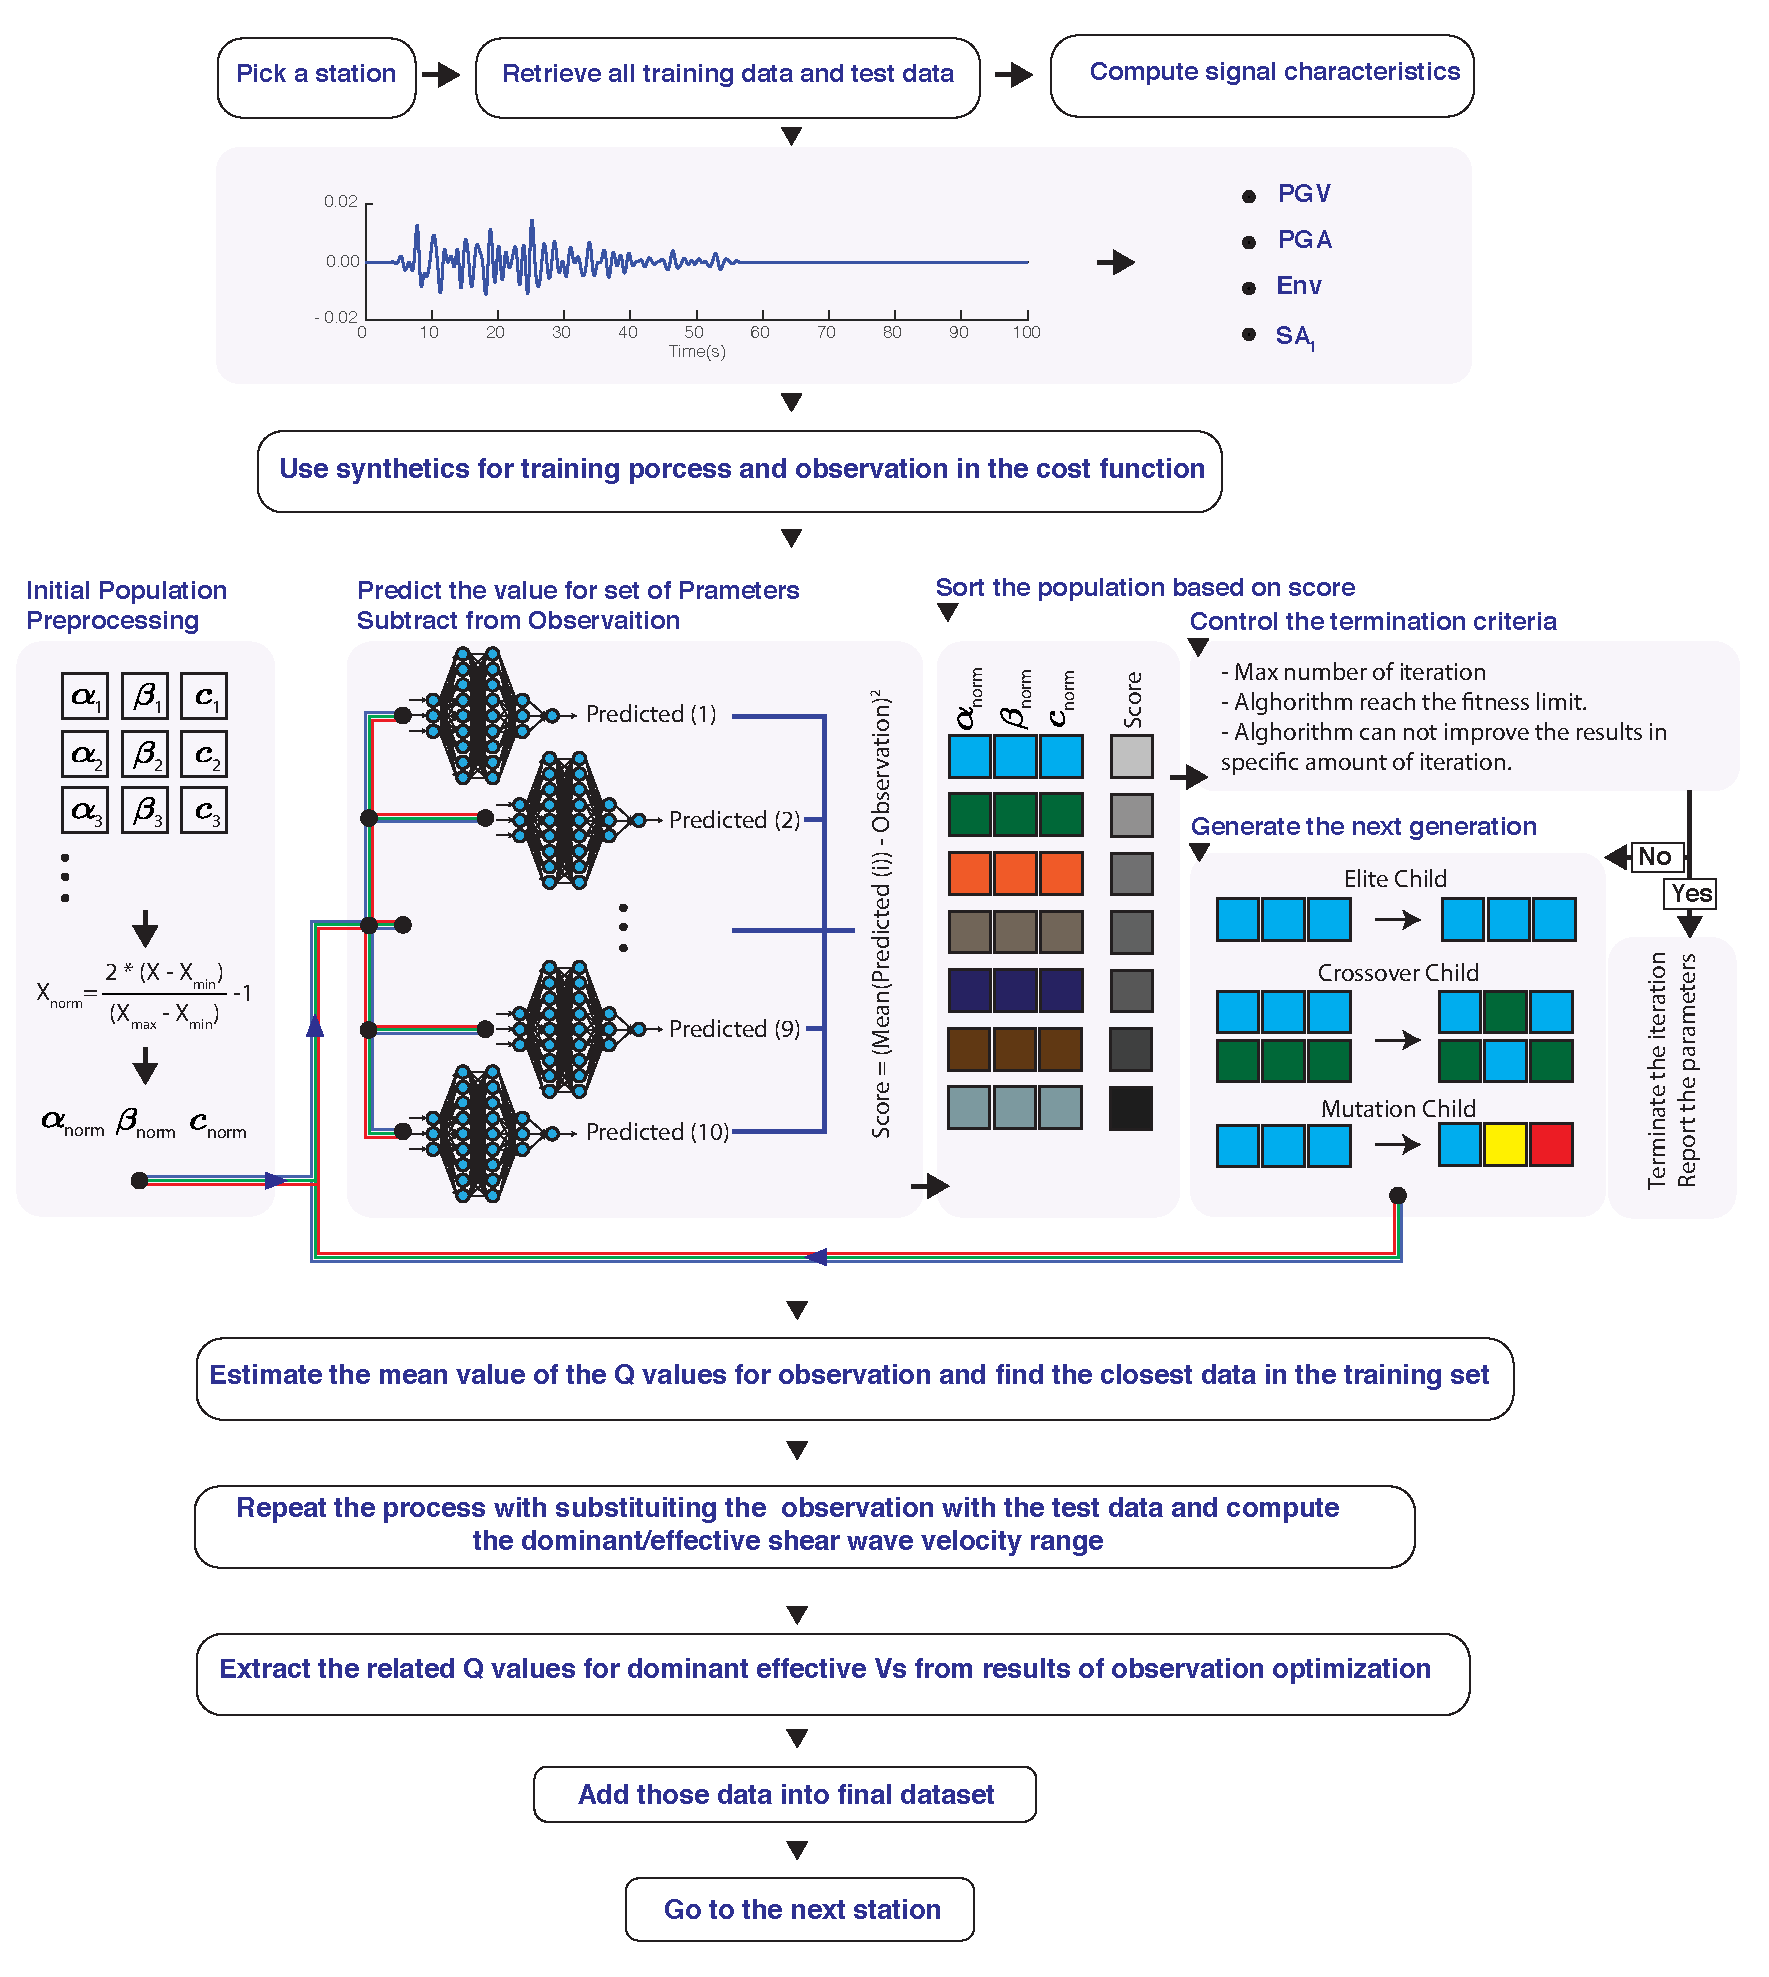
\includegraphics[width=\textwidth]{figures/pdf/Figure_02.pdf}
    \caption{Processing steps {\color{red} working on improving this figure and the caption.}}
    \label{fig:Figure_1}
\end{figure}

In the rest of this section, we go into details of each mentioned tasks.

\subsection{Attenuation models and ground motion simulations}
We use a finite element code to conduct physics based ground motion simulation \citep[for more details see ][]{Tu_2006_Proc,Taborda_2010_Tech}. 
In the code, energy loss due to anelasticity is represented by springs and dashpots. In this study, we use a model which combines two Maxwell elements and one Voigt element \citep{Bielak_2011_G}. The model converts the provided $Q$ value to desirable attenuation in the forward simulation. For the $Q$ equation we use the following equation: 

\begin{equation}
Q_{S}(V_{S}) = C + \alpha(V_{S})^{\beta}
\end{equation}

$C$ serves as floor value for low-velocity structures and $\alpha$ and $\beta$ offer different growth rates for increasing values of \vs{}. \qp{} depends on \qs{} and \qk{}, which is dilatational reciprocal quality factor. Since in soil and rock materials the intrinsic attenuation due to shear is generally much greater than that due to dilatation, we ignore dilatational reciprocal quality factor (\qk{}=~$\inf$). \qp{} is computed using

\begin{equation}
Q_{P}=2Q_{S}.
\end{equation}

Based on random combination of \qsvs{} relationship input parameters (i.e., $C$, $\alpha$, $\beta$) we run many physics-based ground motion simulation and generate the training dataset. 

\subsection{Signal Metrics}

There are numerous methods for quantitatively comparing two signals in time and frequency domain (see khoshnevis and Taborda 2018 and references therein). Q factor parameter studies commonly use peak ground velocity or peak amplitude of S wave arrivals as an indicator to energy loss during the wave propagation. Unless in a completely homogenous domain, it is not easy to pick the peak ground velocity for S-wave arrival. In a complex geological structure surface wave and  direct S wave and reflected body waves from different layers are mixed together. In that case the energy is already dissipated in propagation process and the peak ground velocity is not very sensible to the Q parameters. We will have more discussion on this issue in the result section. Also picking the actual peak value of S Wave arrivals is extremely prone to error and it is not straight forward to distinguish body wave and surface wave windows in a complicated geological regions \citep[e.g., see][]{bowden2017earthquake}. Moreover, our ideal case experiments prove that using only peak ground velocity will not necessarily provide better results even if we be able to accurately pick the peak ground velocity for S wave. Khoshnevis and Tabarda 2018 showed that response spectra is the most important parameter in qualitative comparison of signals as well as total energy. Following their recommendation, in this paper, we add 3 other parameters to the qualitative comparison of signals process. Keeping peak ground velocity, we also use response spectra for the highest frequency of the simulation ($T= 1s$), peak ground acceleration and area under the envelope of the signal which is another indication of total energy. For more details about the GOF metrics please refer to  khoshenvis and Taborda 2018. We computed the signal envelop using the Hilbert transform. Figure.~\ref{fig:signal_envelop} Shows example of signal envelop and the area under it. 

  \begin{figure}[ht]
    \centering
    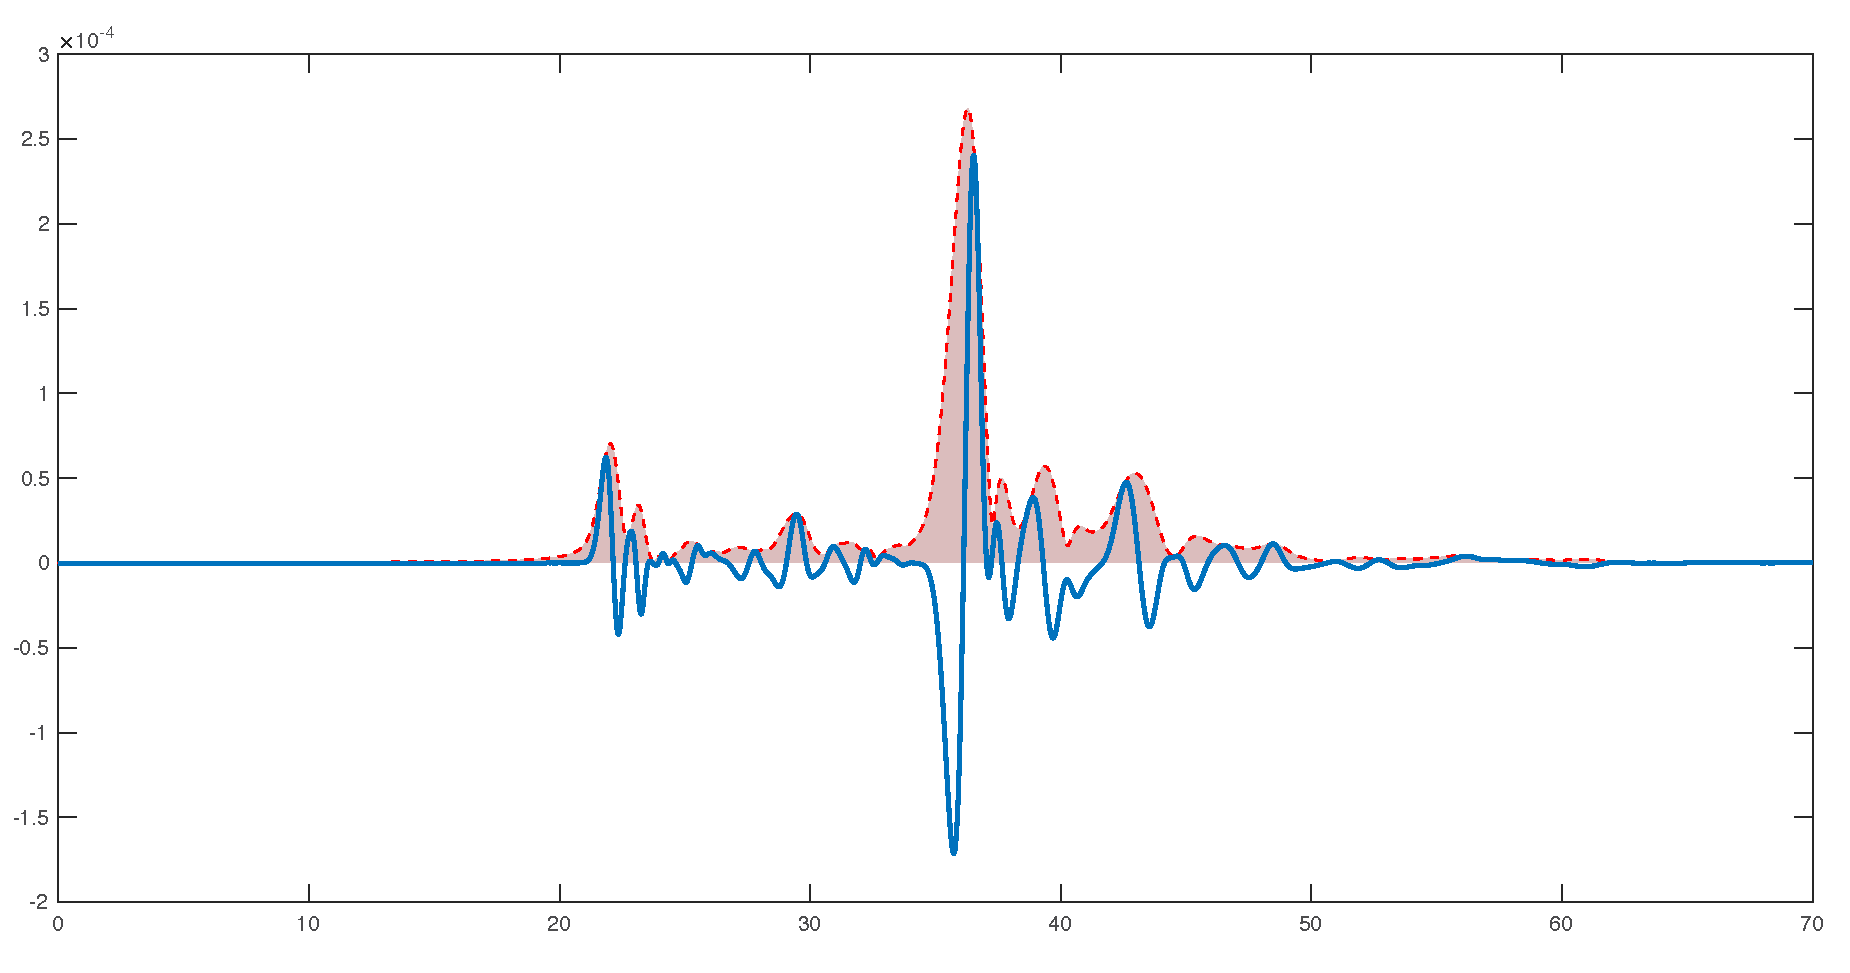
\includegraphics[width=\textwidth]{figures/pdf/signal_envelop.pdf}
    \caption{Example of signal envelop}
    \label{fig:signal_envelop}
\end{figure}




\subsection{Developing surrogates} 

Surrogates are developed using artificial neural networks (ANNs). ANNs are inspired in the human brain. A given network is a combination of different so-called neurons which have certain initial weight and activation functions. These neurons are grouped in different layers. The first layer is called input layer, and the last layer is called the output layer. Other layers between input and output layers are called hidden layers. We use two structures of ANNs.  One structure is developed to estimate PGV, and the other structure is developed to estimate PGV, PGA, SA, and Venv for two horizontal components. Alternative metrics increase signal uniqueness. There is less chance that two signals which are generated with two sets of different input parameters (i.e., $C$,$\alpha$, and $\beta$) have the same PGV, PGA, Venv and SA. Consequently, the optimization algorithm can effectively find the best set of solutions. Fig.~\ref{fig:Figure_ann_structure} shows the structures of networks. The number of neurons in each hidden layer is presented at the top of each layer.

 \begin{figure}
    \centering
    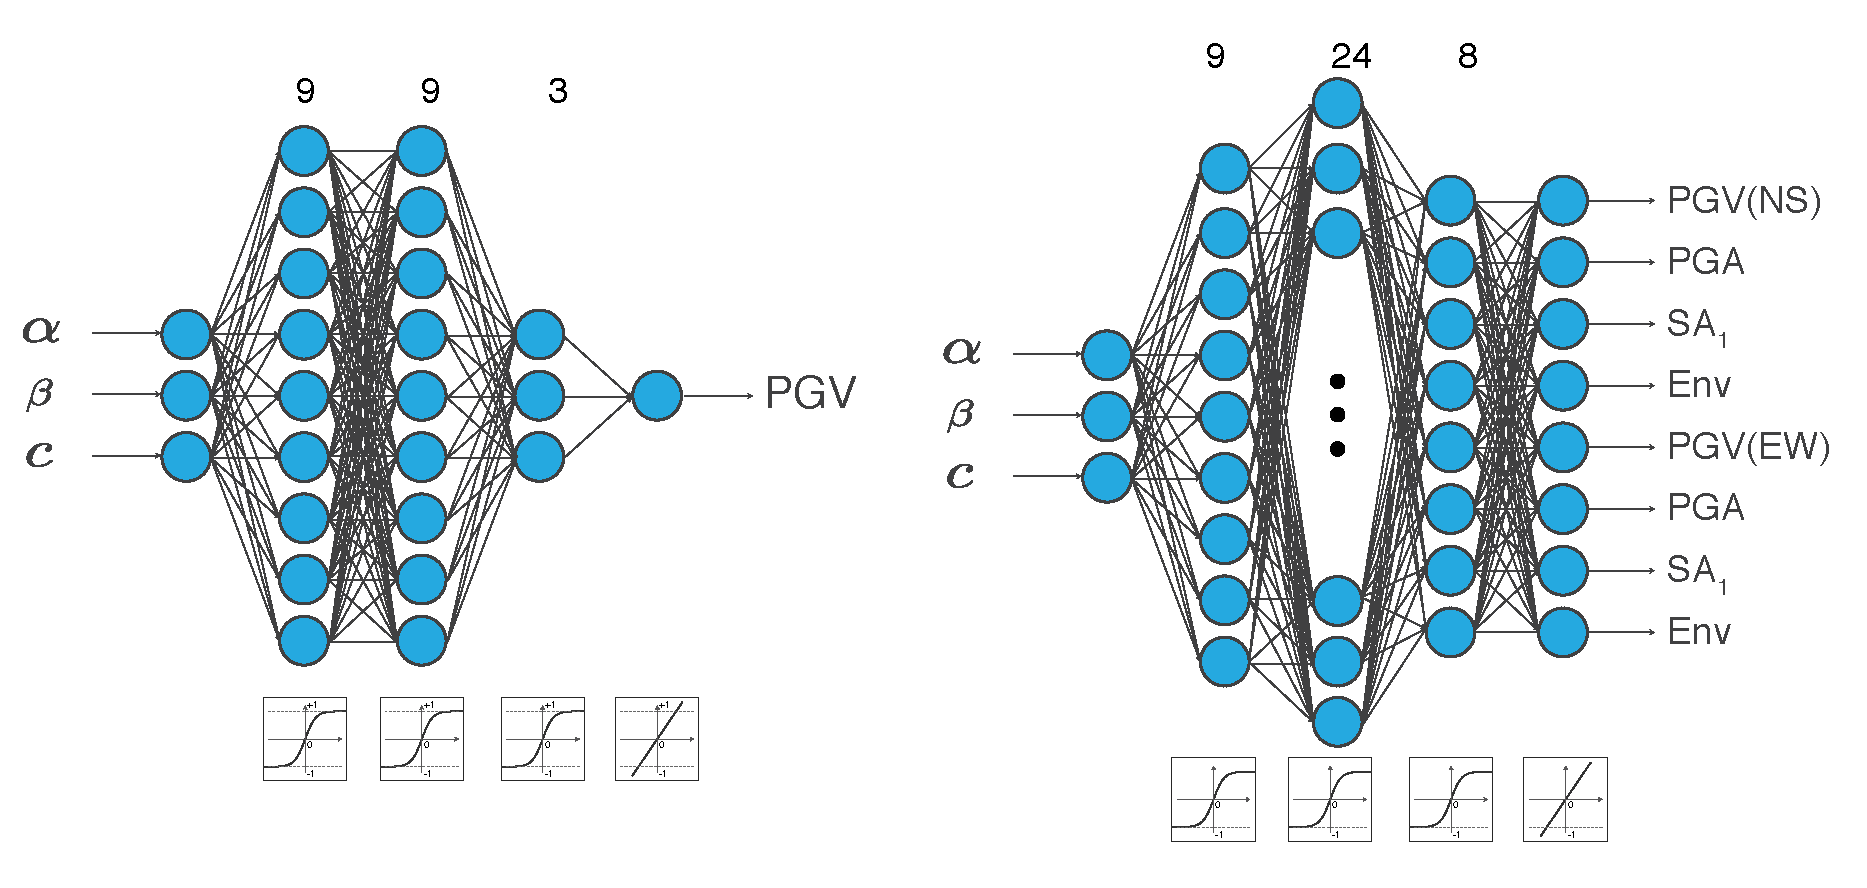
\includegraphics[width=1\textwidth]{figures/pdf/Figure_03.pdf}
    \caption{Feedforward multilayer perceptron neural networks used in the study. Hidden layers use tangent sigmoid and output layer uses linear activation functions. Dots used to simplify the structure for presenting purposes.}
    \label{fig:Figure_ann_structure}
\end{figure}

Input values for all ANNs in this study is \qsvs{} relationship parameters (i.e., $C$, $\alpha$, and $\beta$). All nodes are interconnected, and each layer has an activation function. One can train a network using available data by means of a process during which the weights and bias values associated with the network's neurons are updated so that these will produce output results with increasingly lower residuals in comparison with the input observations. Training ANNs provides a mean to avoid repeated expensive computations. Studying neural network structure and different networks and algorithms are beyond the scope of this study.  In this study, we use feedforward neural networks and Levenberg-Marquardt optimization as a network training function to update weight and bias values. We use linear transfer functions for the last layers and hyperbolic tangent-sigmoid transfer functions for the rest of them. The package is implemented in Matlab programming tool. The algorithm divides the data into three sets including training, validation, and testing dataset. Validation dataset is used to stop training process to avoid overfitting during the training process. An ANN can accurately learn any dataset, provided there is no noise in the data. However, a well trained ANN for one dataset may not be a good predictor for another dataset. This situation is called overfitting. Validation dataset is used to stop the training processing when overfitting occurs. The test dataset is used after fully training data to analyze the functionality of the network. For training ANNs, first, we leave out 5\% of the dataset for the final testing. These data have never been provided to ANNs during the training sessions. We assign 85 and 15\% of remaining data into training and validation datasets.  Neural networks' training process, depending on the size of the networks, is involved with hundreds of thousands of matrix multiplication. Therefore, normalized input values ensure the stability of the networks and improve its internal optimization process in case of inequivalent attributes. We linearly scale the data into $[-1,1]$ using

\begin{equation}
X_{norm} = \frac{2*(X-X_{min})}{(X_{max}-X_{min})}-1
\end{equation}

where $X_{norm}$ is the normalized value; $X_{min}$ and $X_{max}$ are minimum and maximum value of $X$ vector, respectively. The performance is computed by use of mean squared error (RMSE) between the network predicted values and observation. As of epoch number increases, the network learns to predict the data with high accuracy. An epoch is one complete presentation of the dataset to be learned to an ANN. For a small dataset where all data can fit into the system at once, one epoch is one iteration. In general, with increasing training data, the network functionality increases for unseen data and becomes more generalizable. Generalizability means that the trained ANN can accurately estimate the output values from input values that it has never seen them before. In many cases, developing training data can cost a considerable amount of computational and financial resources. Studying the methods for generating the most appropriate training data is beyond the scope of this paper. In this study, we generate enough training data and study the effect of training data size in network performance. We use bootstrap aggregating (bagging) predictors to increase the generalizability and accuracy of predictors \citep{Breiman_1996_ML}. Bagging is a method for generating multiple versions of a predictor and using these to get an aggregated predictor. We use the trained networks in optimization process as surrogates in the cost functions. 




\subsection{Optimization process}

Having the boundaries of parameters and a cost function, we need to set up an optimization process to search for the best set of parameters to efficiently minimize the cost function. Our preliminary studies (include 2016 scec poster) show that there are not a unique solution for the process and many combination of parameters can be a good candidate. It is understandable because for each station there is a dominant shear wave velocity  in the ray path. Therefore, different combination of parameters where they generate common values for a range of Vs can be acceptable results. Therefore, our cost function can have infinite number of local minimum with acceptable accuracy. In result we need to have a global optimization process to be able to have a good searching strategy in different part of the domain.  Therefore, we use Genetic algorithm as a derivative free single objective method in optimization process. We generate a series of optimal results for each station. These results provide a good understanding of the dominant/effective shear wave velocity for that specific station. \\

\citet{Holland_1973} introduced genetic algorithms (GA). It is not a mathematically guided solution to the problem; rather, It is merely a stochastic, discrete, nonlinear, and highly dimensional search algorithm.We developed a simple GA according \citet{man1996genetic}. Each population includes the quality factors parameters. After evaluating the first set of populations that are basically random parameters in the defined range, the algorithm iteratively defines new populations. Every time that new population is generated it goes through the evaluation process. In the evaluation process which we call it cost or objective function (according to GA nomenclature), it gets the parameters as an input and compute the differences between observation and synthetic. Then it sorts the population according to the best cost (in ascending order). In order to facilitate the GA evolution cycle, two fundamental operators: Crossover and Mutation are required. We use uniform crossover approach as crossover operations. This generates offspring from the parents based on randomly generated crossover mask. 
In this process for each iteration, and for each population, parents exchange the sections to generate the offspring.  At each iteration also in the mutations process, the algorithm randomly picks new value in the defined range. Crossover tends to conserve the genetic information present in the strings. Mutation however is not a conservative operator but capable of generating new building blocks radically. Upon generating new population the algorithm calculate the costs and sorts the population according to score and crossover the best solution with part of other good solutions. Since the best chromosome of the population may fail to reproduce better offspring in the next generation, it is usually combined with elitist strategy such that one or number of the best chromosome can be copied in to the succeeded generation.  Next generation (offspring) is combination of best solutions of previous generation, mutated generation and crossover generation. The cycle of evolution is repeated until a desired termination criterion is reached. In this study we use adaptive feasible and crossover scattered functions as mutation and crossover functions (for more details see \citet{Matlab_optim}).  We defined three termination criteria. Maximum number of iteration, in this case the optimization process regardless of the wellness of the results is terminated,  Fitness limit, in this case the value of fitness function for the best point in the current population is less than or equal to fitness limit; and achieving best score and successive iterations with no produce of better results. 

%In this study the we use the default mutation function (Adaptive Feasible) when there are constraints, randomly generates directions that are adaptive with respect to the last successful or unsuccessful generation. The mutation chooses a direction and step length that satisfies bounds and linear constraints.
%Crossover function (CrossoverFcn) specifies the function that performs the crossover. Do not use with integer problems. You can choose from the following functions:
%Scattered (@crossoverscattered), the default crossover function for problems without linear constraints, creates a random binary vector and selects the genes where the vector is a 1 from the first parent, and the genes where the vector is a 0 from the second parent, and combines the genes to form the child.

%        PopulationType: 'doubleVector'
%             PopInitRange: [2�3 double]
%           PopulationSize: 40
%               EliteCount: 2
%        CrossoverFraction: 0.8000
%           ParetoFraction: []
%       MigrationDirection: 'forward'
%        MigrationInterval: 20
%        MigrationFraction: 0.2000
%              Generations: 20
%                TimeLimit: 600
%             FitnessLimit: 1.0000e-04
%            StallGenLimit: 50
%                StallTest: 'averageChange'
%           StallTimeLimit: 300
%                   TolFun: 1.0000e-06
%                   TolCon: 1.0000e-03
%        InitialPopulation: [1 0.8995 -1]
%            InitialScores: [0�1 double]
%       NonlinConAlgorithm: 'auglag'
%           InitialPenalty: 10
%            PenaltyFactor: 100
%             PlotInterval: 1
%              CreationFcn: @gacreationuniform
%        FitnessScalingFcn: @fitscalingrank
%             SelectionFcn: @selectionstochunif
%             CrossoverFcn: @crossoverscattered
%              MutationFcn: @mutationadaptfeasible
%                  Display: 'final'
%               Vectorized: 'off'
%              UseParallel: 1
%     UserSpecPopInitRange: 0
%           MultiObjective: 0
%                Verbosity: 1


\subsection{Effective Shear Wave Velocity Range}

There is not a unique solution for \qsvs{} input parameters. Many combinations of the parameters can provide similar $Q$ and, consequently, accurate results. Although we define the anelasiticy as a function of the shear wave velocity, ground motion simulation model generates a Q value based on provided input parameters. As an example if we consider a domain with \vs{}=1500~m/s, and $Q=$~120 which is measured for the region, all the \qsvs{} relationships that are shown in Table~\ref{tab:example_effective_vs} are considered acceptable. 

\begin{table}[ht]
\centering
\caption{Example of acceptable parameters for  a domain with $Q$~=120 and \vs{}=1500~m/s}
\label{tab:example_effective_vs}
\begin{tabular}{ccc}
C  & $\alpha$ & $\beta$ \\ \hline
5   & 20                    & 4.3141               \\
10 & 25                    & 3.6541               \\
15 & 30                    & 3.0897               \\
20 & 35                    & 2.5892               \\
25 & 40                    & 2.1333              
\end{tabular}
\end{table}

Fig.~\ref{fig:example_acceptable_parameters} illustrates Table~\ref{tab:example_effective_vs} parameters. For ground motion simulation models only $Q$ value (which is 120 in this example) is important. Obviously, infinite combination of parameters can generate the objective $Q$ value. 

 \begin{figure}[ht]
    \centering
    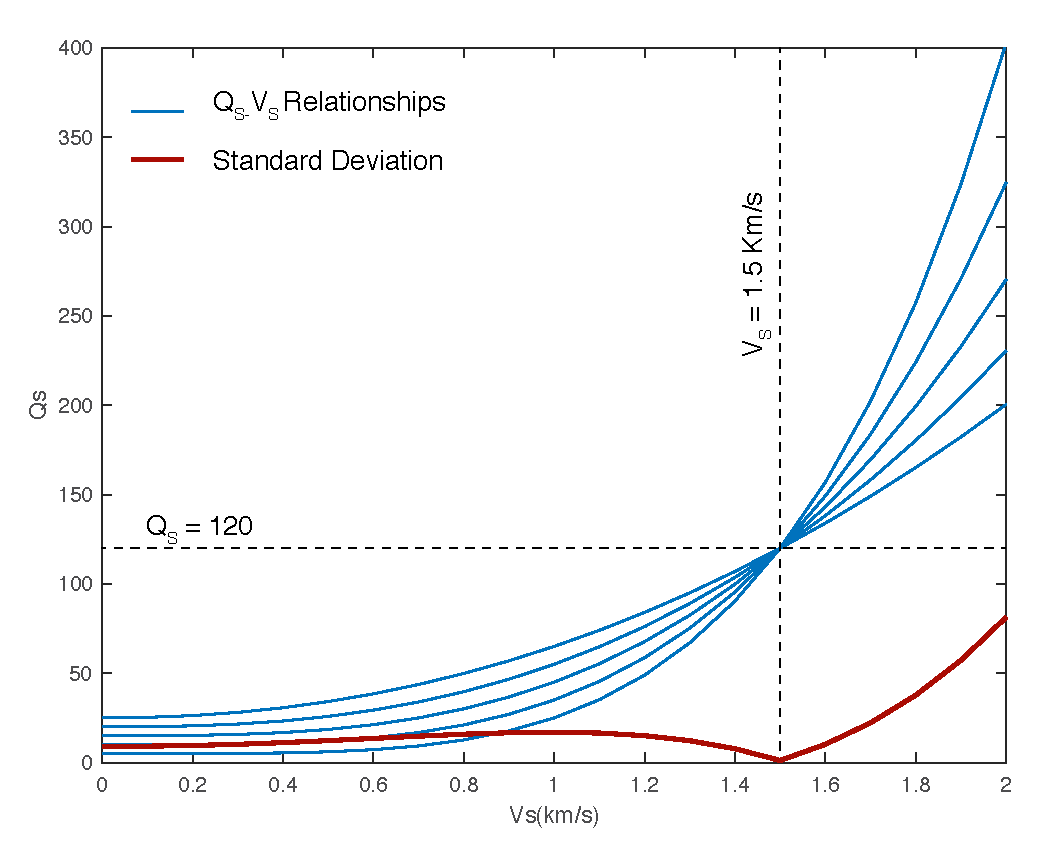
\includegraphics[width=0.5\textwidth]{figures/pdf/Figure_04.pdf}
    \caption{Example of acceptable solutions for constant \qs{} value. Blue thin lines are plotted based on Table~\ref{tab:example_effective_vs} parameters. Red thick line is standard deviation of \qs{} values. Standard deviation is the minimum value at the convergence point.}
    \label{fig:example_acceptable_parameters}
\end{figure}

Therefore, the optimization process, with respect to the shear wave velocity range of each station will find a set of appropriate parameters. With repeating the optimization process and plotting the results, we indicate the effective shear wave velocity range by computing standard deviation of the $Q$ values for each \vs{}. Standard deviation, in this context, is a proxy to measure the level of convergence. We consider two main conditions to accept the results of optimization processes:

\begin{itemize}
\item If synthetic solutions converge at a range of shear wave velocities
\item If the optimization process successfully locate the input parameters
\end{itemize}
 
 Application of standard deviation can address the first condition. The second condition is the research question of this study. We do not know the $Q$ values for the study region. However, we can follow several steps to estimate the capability of the optimization process.  The mean value of all converged solution can be considered as a potential answer to the research question because it has the same values at the convergence point as other solutions. Therefore, We use that $Q$ values and run ground motion simulations and assign the results as a target value. This time we run the optimization process with the new target value. If the converged points are the same as initial parameters (i.e., $Q$ values according to used $C$, $\alpha$, $\beta$ for target simulation), we accept the first results that come from optimization process for actual observation. If the convergence points and used $Q$ values do not coincide we reject the solutions. In other words, we study whether the optimization process is capable of finding appropriate parameters while the target $Q$ is close to mean $Q$ values. Some stations provide a convergence point different than actual parameters. One reason can be the metrics that we use. Maybe they are not adequate for some stations signals. More research is ongoing in this section. Whatever the reason is, if we do not trust the process for a specific station, we ignore the results of the process. 
 









\section{ Test Scenarios and Study Region}

We tested the proposed method on four different idealized domains and a real heterogenous domain. The idealized domains are homogeneous and layered. Figure.~\ref{fig:3d_domain_scenarios}  represents these domains. 

 \begin{figure}[ht]
    \centering
    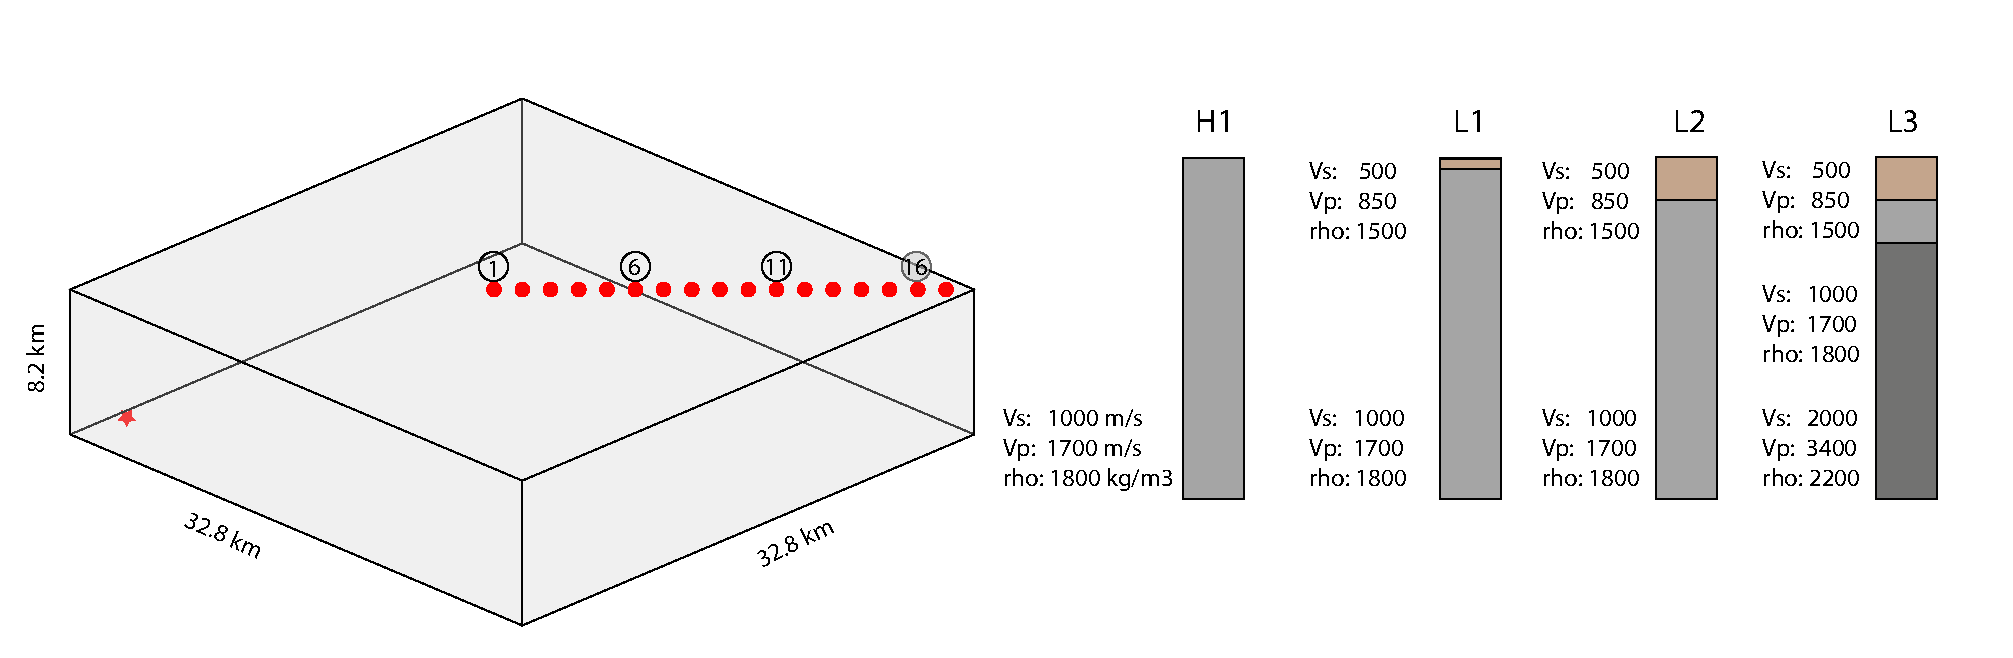
\includegraphics[width=\textwidth]{figures/pdf/3d_domain_scenarios.pdf}
    \caption{Idealized domains to test the proposed method.}
    \label{fig:3d_domain_scenarios}
\end{figure}

Testing of the proposed method is inspired from checker board test idea from inversion studies (add some references). We develop an artificial domain with  known damping parameters, and using the observed data at each stations we search for the initial used parameters. The real heterogeneous region  has greater Los angeles area and also it includes many small basins in different parts. Numerous earthquake recorded in this area and different studies is conducted from different perspective.  Several velocity models are developed and it in an going process \citep[e.g., see][]{small2017scec}. Fig.~\ref{fig:Figure_stations} shows the  heterogeneous domain and stations location. 

 \begin{figure}[ht]
    \centering
    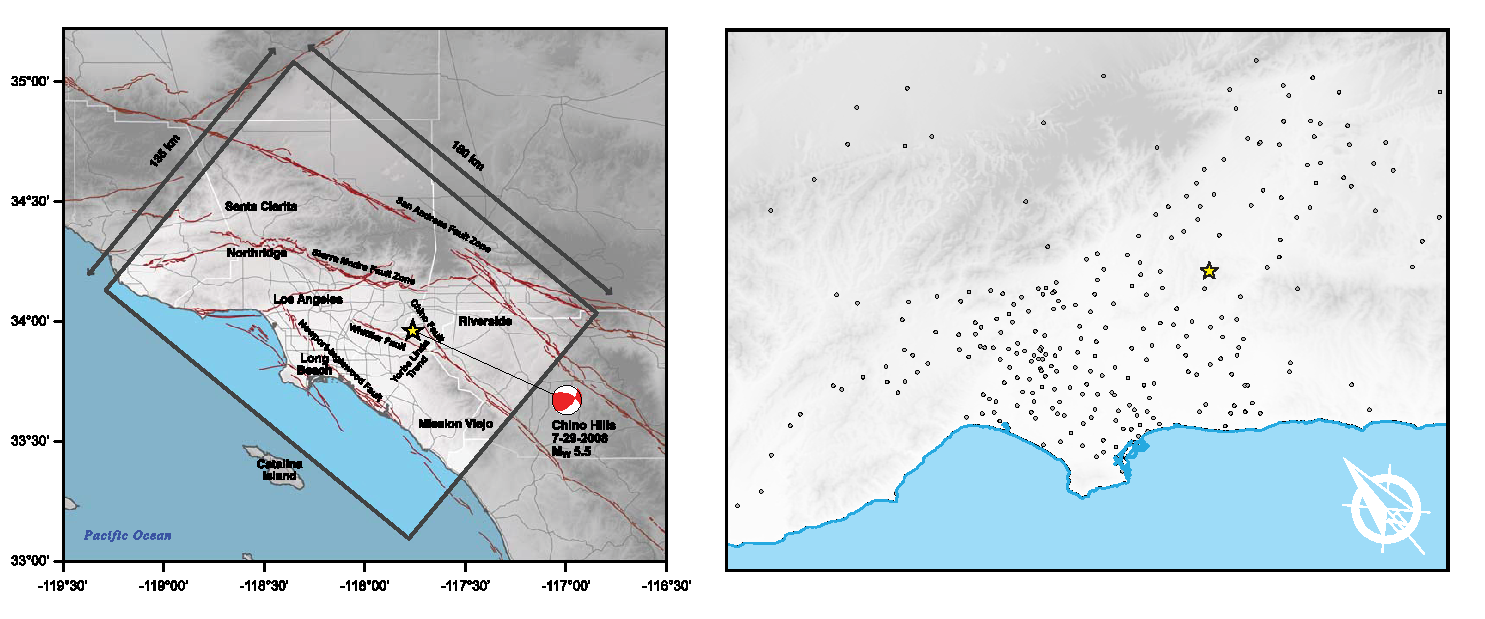
\includegraphics[width=\textwidth]{figures/pdf/Figure_stations.pdf}
    \caption{Processing steps}
    \label{fig:Figure_stations}
\end{figure}


In order to test the methodology with real observational data, we use 2008 $Mw~5.4$  ChinoHills earthquake as an observation platform. Chino Hills earthquake is recored in more than 300 stations. however we only use the strong motion center stations, where in our study simulation box there are 262 stations.  Table.~\ref{tab:event_details}  and Table. ~\ref{tab:sim_param} represent the event and simulation details, respectively. 


\begin{table}[ht]
\centering
\caption{Event details}
\label{tab:event_details}
\renewcommand{\arraystretch}{0.75}
\begin{tabular}{lr}
\\ \hline
Name                                 &   Chino Hills                          \\
Origin Time                        & 29 July 2008 , 11:42 AM             \\
Magnitude                          &  Mw 5.4            \\
Moment                             & 1.566751e+17 Nm             \\
Location/Depth                  &  -117.7613 33.9530 14.7 $Km$    \\
Strike/Dip/Rake                 & 47/51/32                                   \\
3D Crustal Model              & SCEC CVM-S4.26                   \\
Source Model                   & Point Source                                  \\ \hline
\end{tabular}
\end{table}


\begin{table}[ht]
\centering
\caption{Simulation Parameters}
\label{tab:sim_param}
\renewcommand{\arraystretch}{0.75}
\begin{tabular}{lr}
\\ \hline
Domain                              &                              \\
~~Length/Width/Depth       & 180,135,61.875 km \\
~~Southwest corner          & -119.288842, 34.120549             \\
~~Northwest corner           & -118.354016, 35.061096             \\
~~Northeast corner            & -116.846030, 34.025873              \\
~~Southeast corner           & -117.780976, 33.096503               \\
~~Rotation Angle               & 39.9 \\
~~Studied records             & 262 \\
Spatial Resolution              &    \\
~~Maximum frequency     & 1 $Hz$ \\
~~Minimum $V_s$            & 350 m/s \\
~~Points per wavelength   & $9\leq p < 14$\\
~~Minimum size element   & 21.9727 $m$\\
~~Maximum size element   & 351.5625 $m$\\
~~Number of elements       & 157209765 \\
~~Number of nodes            & 180080443 \\
~~Number of dangling nodes & 23681911 \\
Time resolution  & \\
~~Simulation $\Delta$t & 0.002 \\
~~Simulation time & 100 s\\ \hline
\end{tabular}
\end{table}





\section{Results}
In this section we test the proposed method on the models. The first idealized domain is a homogenous domain with shear wave velocity of $1000 km/s$. For more information about domain details and stations location see Fig.\ref{fig:3d_domain_scenarios}. Simulation record section shows a very clean arrivals (see Fig.\ref{fig:record_section_1000}.) We train the networks with 1000 set of input parameters. In this case we use PGV of north--south component in optimization process( results for other horizontal components or a combination of them are similar.)  We also generate a set of input parameters as a synthetic observation. The optimization algorithm search for parameters that are the best fit with synthetic observation.  Fig.~\ref{fig:station_1_1000_H1} shows the results of optimization process. For each station we repeat the optimization 50 times. We expect to see at each station, for the effective shear wave velocity (here \vs{}=1000~m/s), the optimized parameters and the target parameters $Q$ are very close to each other if not the same. 

  \begin{figure}[ht]
    \centering
    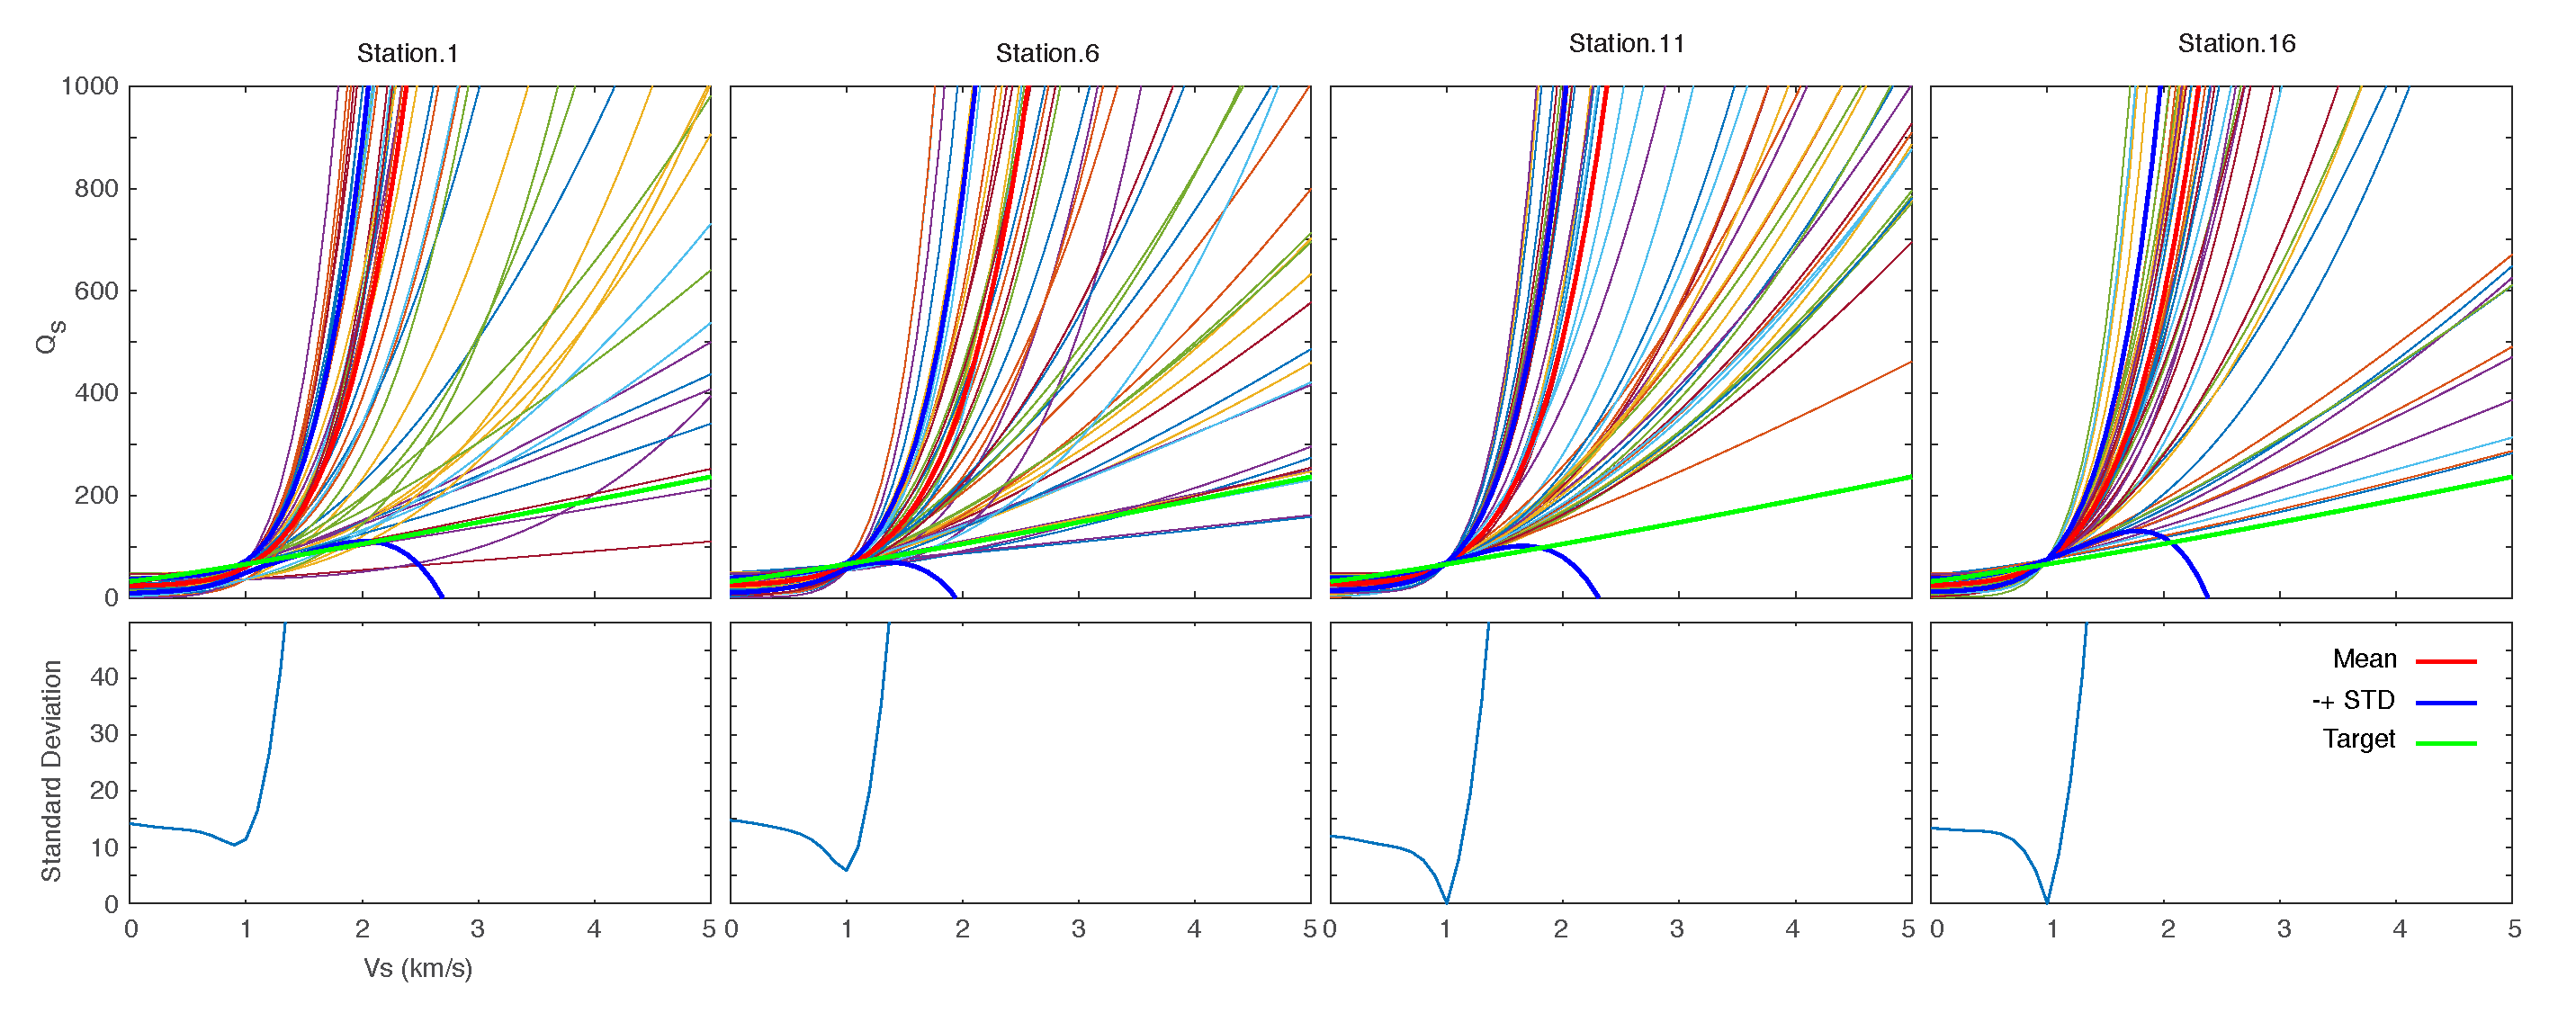
\includegraphics[width=\textwidth]{figures/pdf/Figure_14-H1-pgv.pdf}
    \caption{Results of 50 optimized solutions for homogeneous (H1) domain for 4 stations.}
    \label{fig:station_1_1000_H1}
\end{figure}

This figure shows stations 1,6,11, and 16. Standard deviation values which are shown at the bottom of the each stations are indications of convergence of the solutions. We expect to see a very small standard deviation at \vs{}=1000~m/s. Values of standard deviation is decreased at that \vs{}, however,  only station 11 and 16 have a very converged solutions. That is understandable, because at the closer stations the wave does not have chance to travel enough to capture the anelastic damping characteristics. The parameters that are used to generate the target values are shown with green thick dashed line. The convergence points are coincides with target value parameters at \vs{}=1000~m/s or is very close to it. This test gives the idea that for simple case if we can accurately pick the peak ground velocity, at considerable distance from the source, our optimization process can accurately estimate the $Q$ value for effective shear wave velocity by converging at that point. Also it can locate the $Q$ value with acceptable accuracy.
We add a shallow low velocity zone to the H1 domain. Fig.~\ref{fig:station_1_1000_500_L1} shows the results of optimization process. According to the results, as we observed in the homogeneous domain, the closes station to the source is not well converged, with increasing distance standard deviation decreases and also in mid-distance we can see effective shear wave velocity is in the range of 900--1000~m/s whereas at far stations with respect to the source the effective shear wave velocity is 1000~m/s. Obviously for far stations the wave are propagated more in the high velocity zone and are highly affected from that.   

  \begin{figure}[ht]
    \centering
    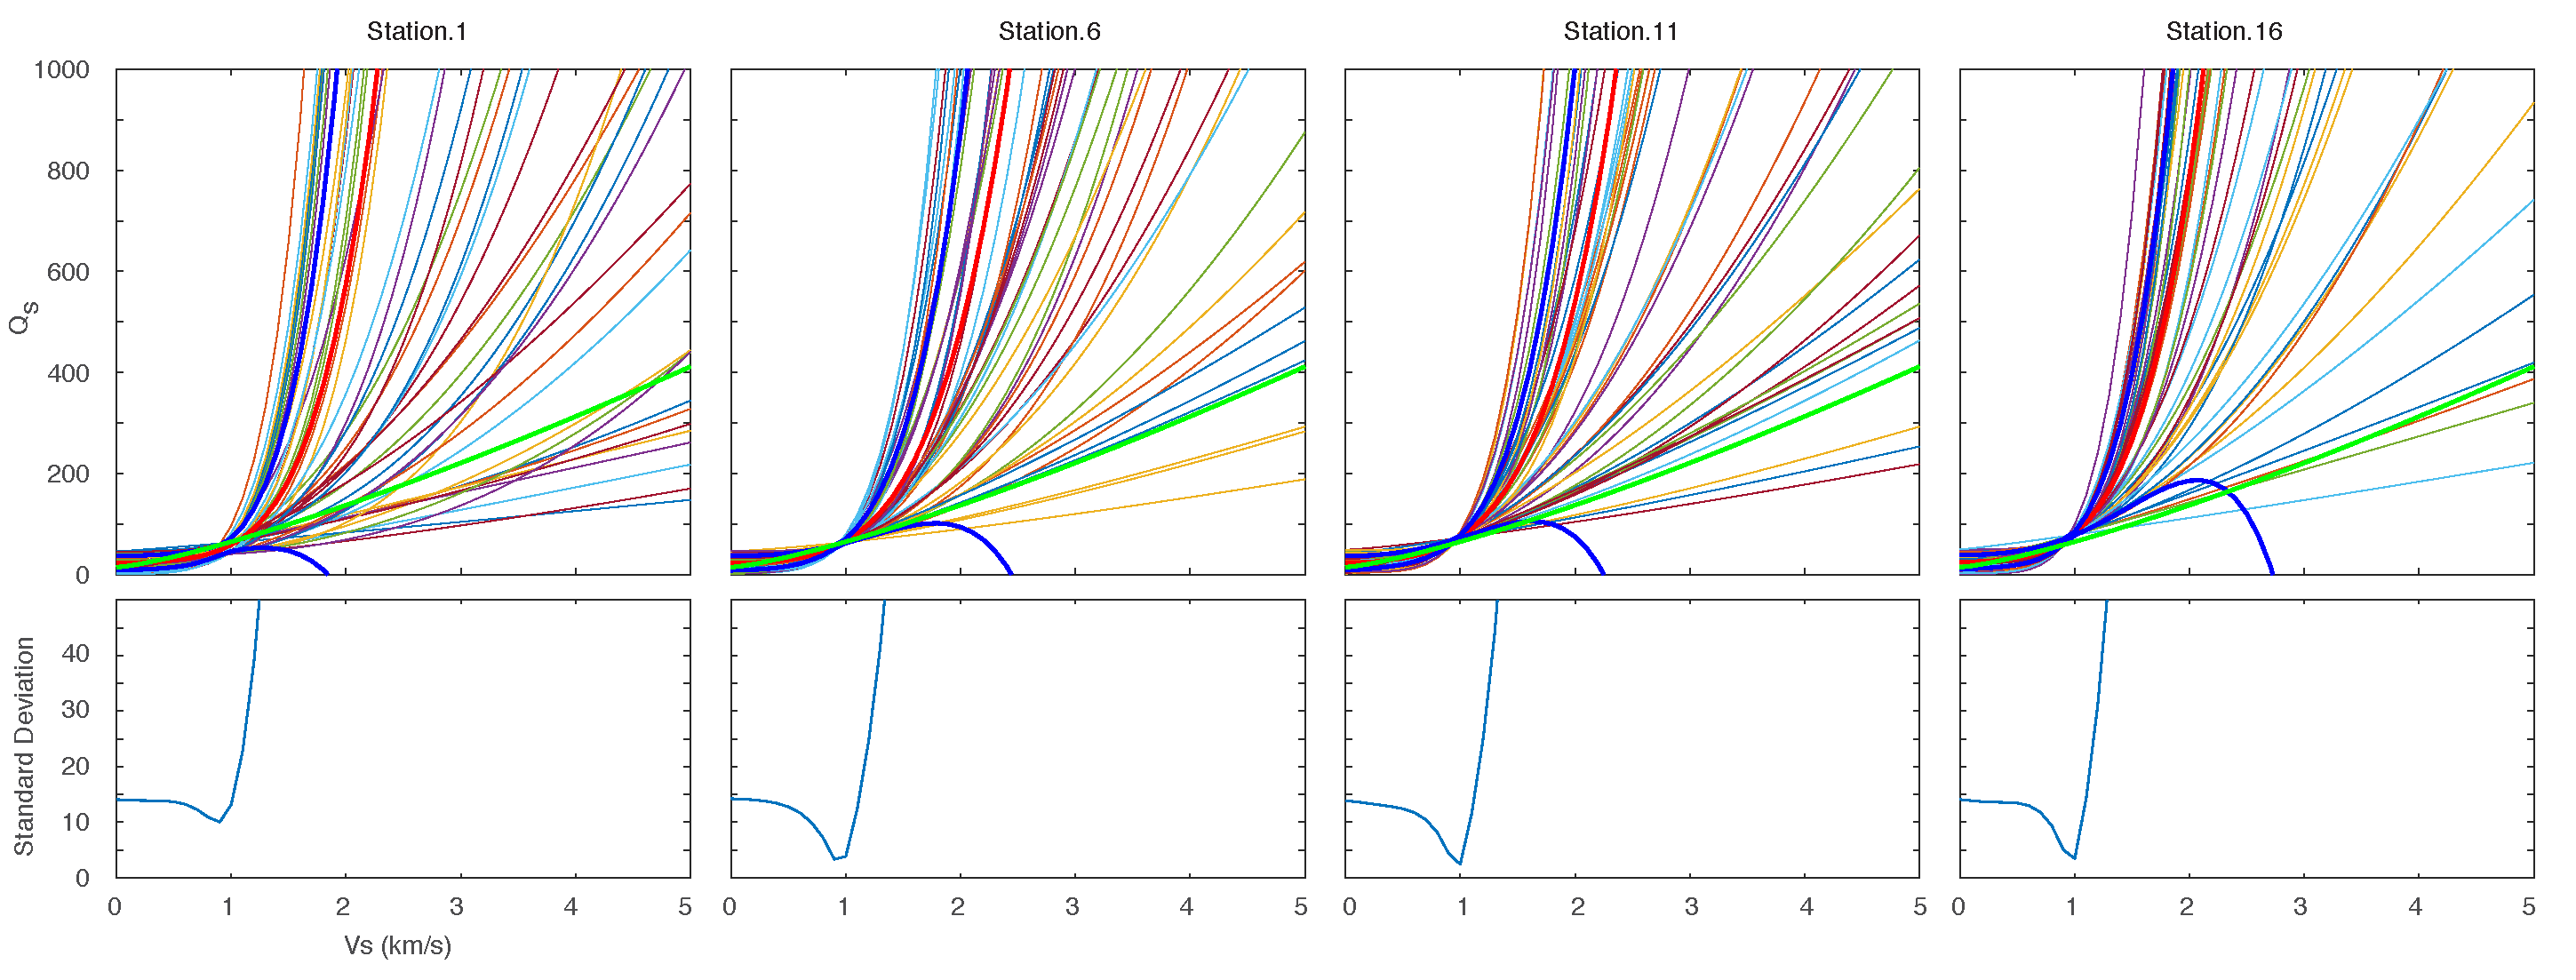
\includegraphics[width=\textwidth]{figures/pdf/Figure_15-L1-pgv.pdf}
    \caption{Results of 50 optimized solutions for Layered (L1) domain for 4 stations.}
    \label{fig:station_1_1000_500_L1}
\end{figure}

It is worth mentioning that effective shear wave velocity that is detected in this idealized scenario is not used in the simulation domain. However, the $Q$ value that is detected for that velocity coincides with the initial \qsvs{} relationship that is used.  The dashed green line is the parameters that we have used for developing synthetic observation values. Ideally, all stations, at their convergence point, should coincides with the line. Station 1 has a very weak convergence rate. Station 6, on the other hand, has a acceptable convergence in solution and also detect the initial parameters (dashed line). Station 11 and 16 have very sharp convergence, but the convergence point has a small difference with initial parameters $Q$ values. According to this results, we can say for this velocity and source model if we use PGV of north--south component as a determining metric, Station 6 most probably will detect the $Q$ parameters.
We increase the depth of low velocity zone of L1 domain (from 256 to 1024 m) to see if the effective shear wave velocities of each stations have considerable changes. Fig.~\ref{fig:station_1_1000_500_2_L2} shows the results of optimization process. The results show that the effective shear wave velocity becomes a little less than $1000~m/s$. It is understandable; because in this scenario the $500~m/s$ low velocity zone can have more effects on propagated waves. In this domain, Station 6 and 11 have good convergence and also could accurately detect the initial $Q$ parameters. 

  \begin{figure}[ht]
    \centering
    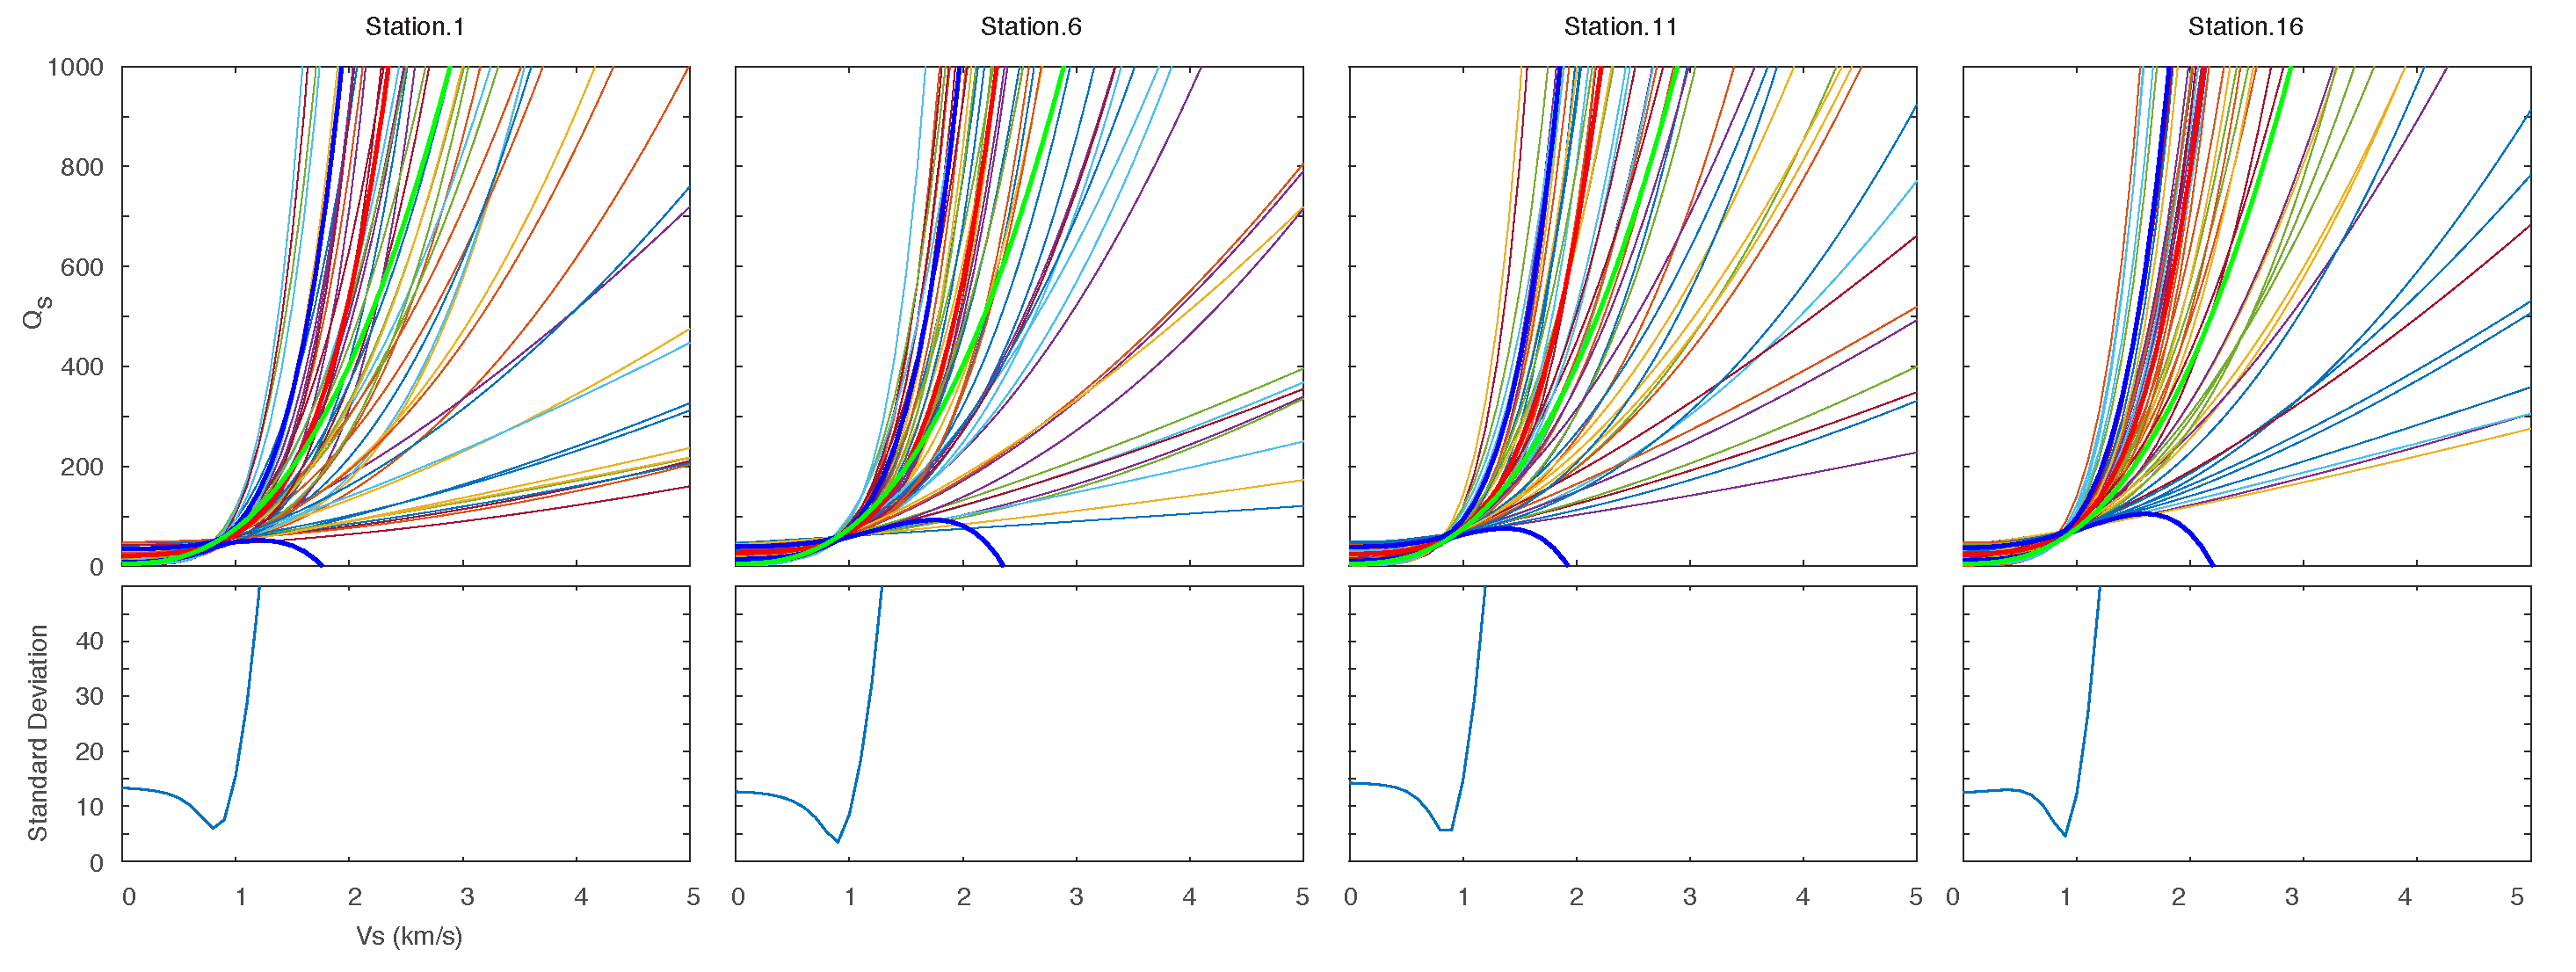
\includegraphics[width=\textwidth]{figures/pdf/Figure_16-L2-pgv.pdf}
    \caption{Results of 50 optimized solutions for Layered (L2) domain for 4 stations.}
    \label{fig:station_1_1000_500_2_L2}
\end{figure}
 

We tried another idealized layered profile with three different layers. According to Fig.~\ref{fig:station_1_2000_1000_500_L3_nt}, with increasing distance from source (Station 1 to 16 ), effective shear wave velocity (i.e., minimum value of standard deviation) is shifting from lower velocity to higher velocity ( m/s to m/s). Far stations records are more affected with high velocity zone. 
 
  \begin{figure}[ht]
    \centering
    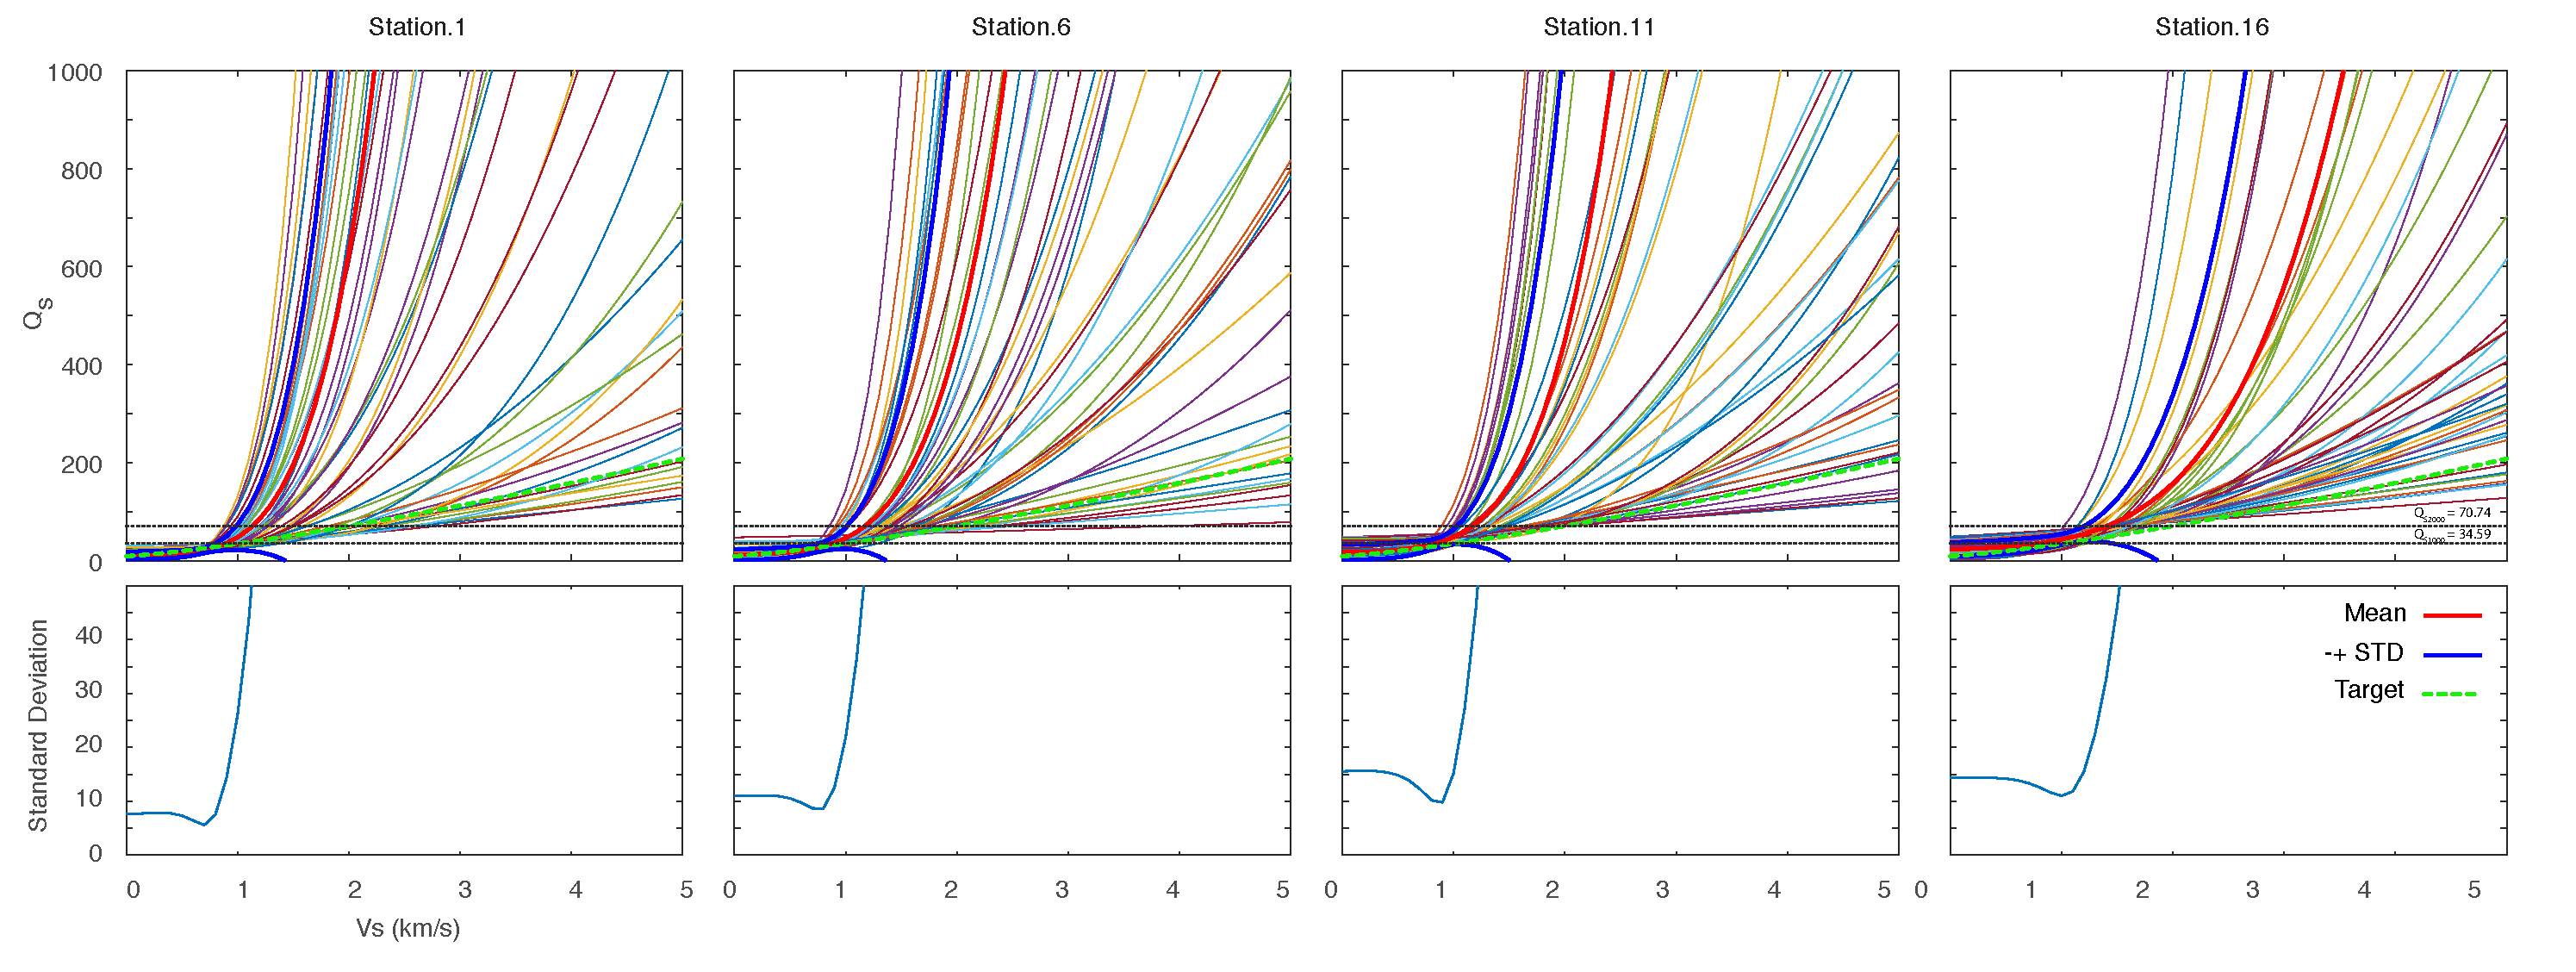
\includegraphics[width=\textwidth]{figures/pdf/Figure_17-L3-pgv.pdf}
    \caption{Results of 50 optimized solutions for Layered (L3) domain for 4 stations.}
    \label{fig:station_1_2000_1000_500_L3_nt}
\end{figure}

However, in this test, we do not see a good convergence rate. The standard deviation of the optimum results around the dominant shear wave velocity is slightly lower, but it is not as sharp as the simpler domains (e.g., H1). We achieved similar results for heterogeneous domain, as well. With increasing domain complexities, determination of effective shear wave velocity is not as sharp as before. It suggests that peak ground velocity may not be enough to estimate the results. Please note that the idealized scenarios do not have noise. Complex geological features (velocity models) make PGV less sensitive to input values. Therefore, we use the second ANN structure where it estimates PGV, PGA, SA1, and Venv for two horizontal components. Fig.~\ref{fig:station_8_param_2000_1000_500} shows the optimization results with using 8 metrics. 

  \begin{figure}[ht]
    \centering
    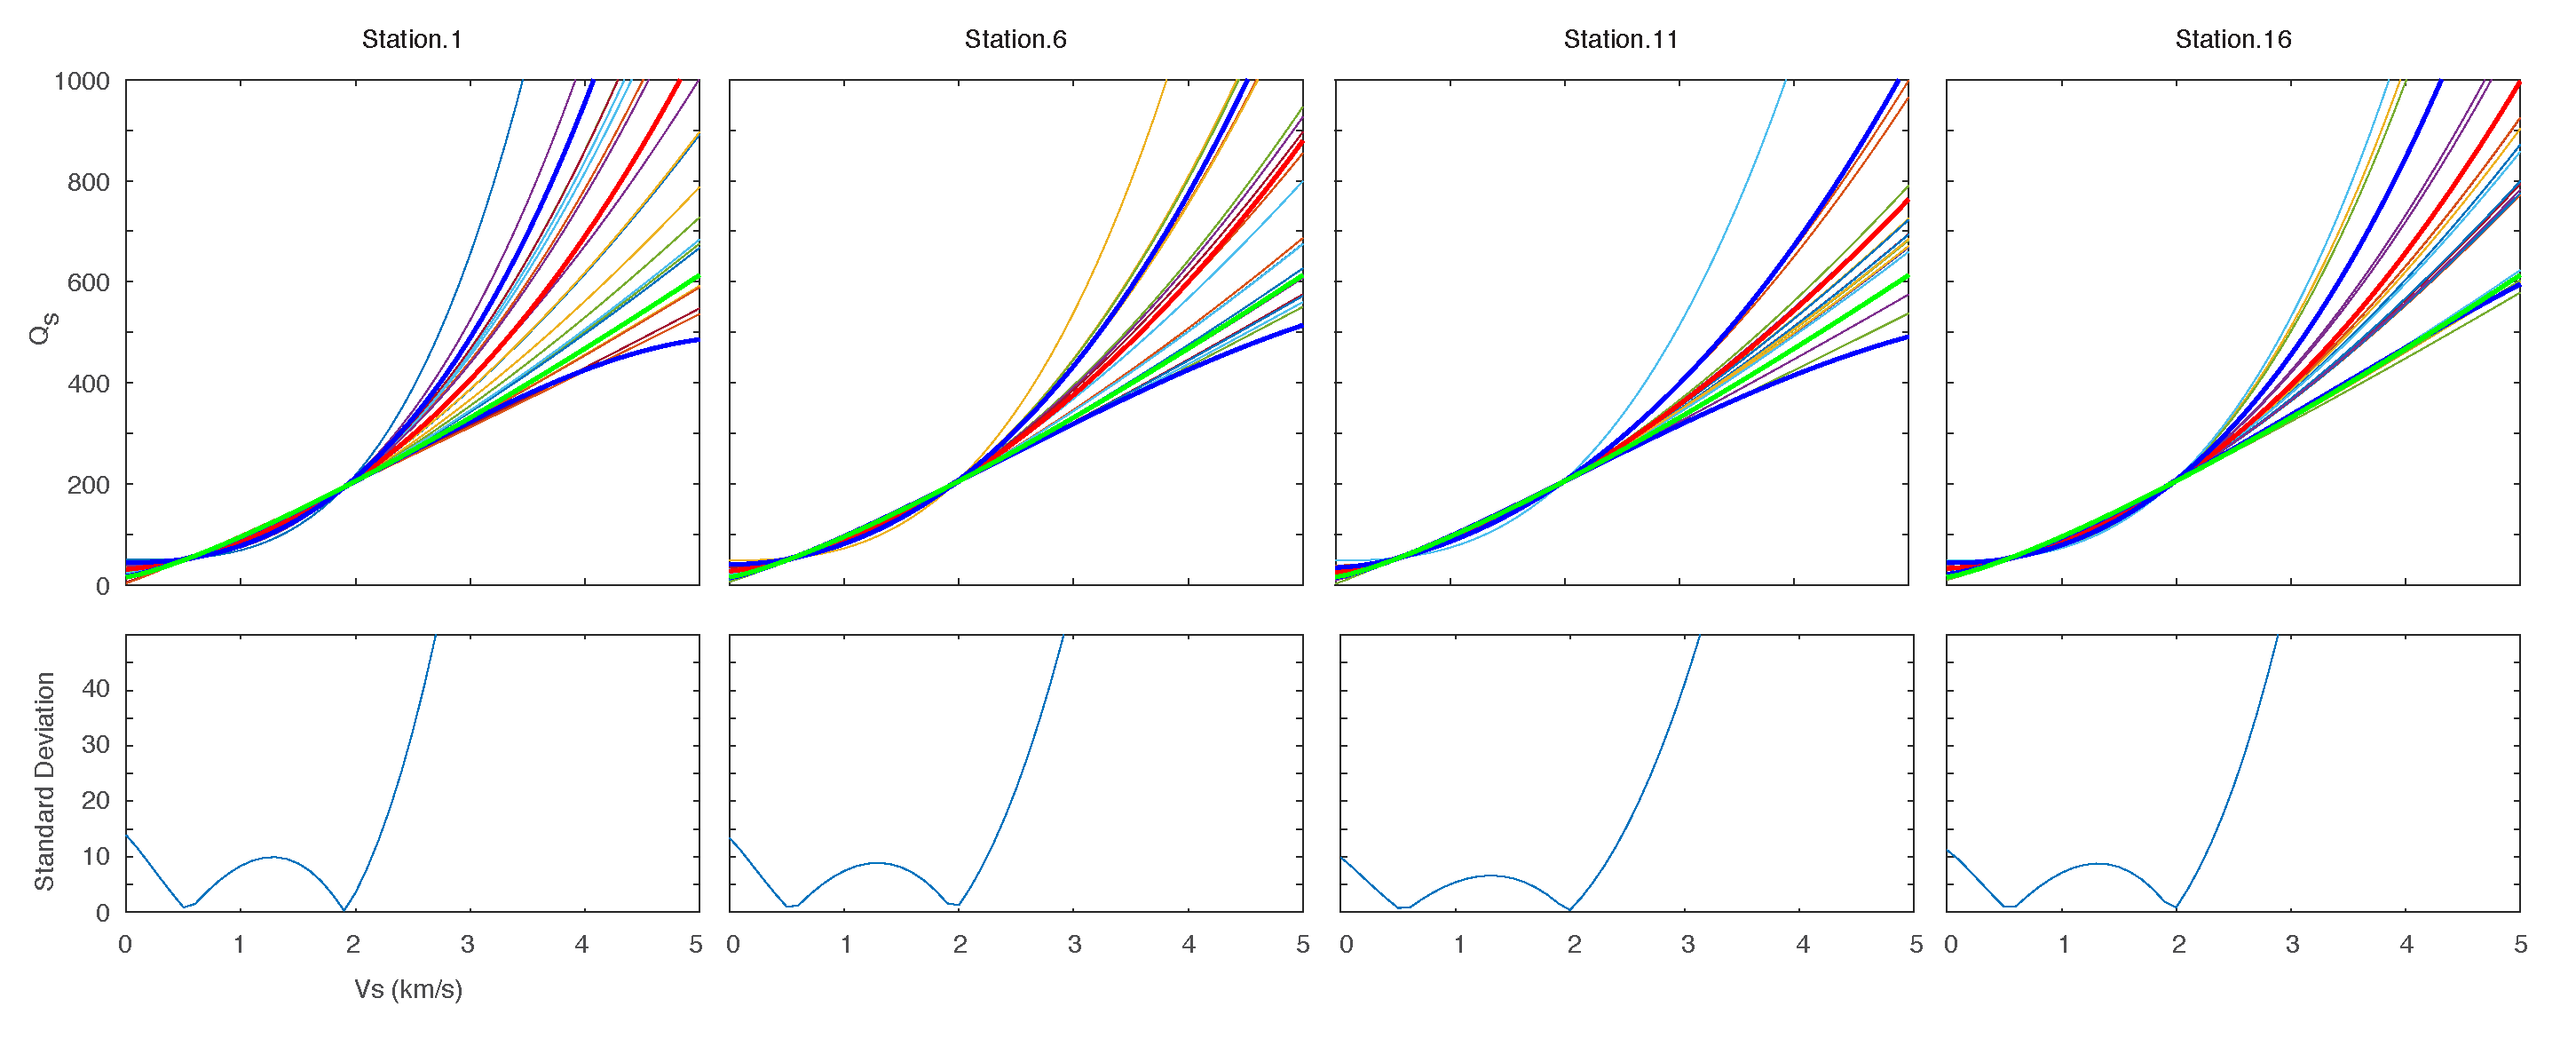
\includegraphics[width=\textwidth]{figures/pdf/Figure_18-L3-8metric.pdf}
    \caption{SA1, PGV, PGA, Env for NS and EW component. Domain(L3).  }
    \label{fig:station_8_param_2000_1000_500}
\end{figure}

There is a significant improvement in the results. The algorithm can locate two ranges of effective shear wave velocities which are 500 and 2000~m/s in all stations. The results are not accurate for 1000~m/s. In this case, the current metrics and problem setup cannot retrieve valuable information for \vs{}=1000~m/s. This does not compromise the proposed method. The positive factor about the proposed method is that we know before hand that we cannot be confident about the results of \vs{}=1000~m/s. However, the results for \vs{}=500 and 2000~m/s are accurate. 
In idealized domains we show that the proposed method can locate a range of effective shear wave velocity and also accurately estimate the $Q$ values. Since idealized domains have up to three different soil layers. At the most elaborate case we will have three $Q$ values with respect to three effective shear wave velocity (in our examples we retrieved at most two effective shear wave velocity ranges.) We can fit a \qsvs{} relationship ($Q=C+\alpha V_{S}^\beta$) which will be similar to any of lines in Fig.~\ref{fig:station_8_param_2000_1000_500}. Obviously, we cannot expect to be able to acquire an accurate results for those shear wave velocity ranges that we have never used in the velocity model. For example in the case of L3 domain, we do not expect to be able to retrieve any accurate data for \vs{}=3000~m/s because the velocity model has 500, 1000, and 2000~m/s.  Therefore, in order to have a comprehensive results, we need to have more \qsvs{} points. In a heterogenous domain, with stations at different places and distance, we can retrieve many data points for different velocity ranges.
We use 2008  $Mw~5.4$ Chino Hills earthquake as a heterogenous domain platform to test the proposed method. The simulation domain and parameters are discussed in the Models Setup section. Fig.~\ref{fig:ANN_accuracy_stations_122_heterogenous_sim_177} shows the accuracy of the neural network for 8 output parameters for a station in the heterogenous medium. According to the figure and RMSE results, ANN can accurately be trained to estimate the requested metrics. We went through all stations, and almost all of them are similar to this station results. Please note that the 50 test data which are used here have never been seen with algorithm during the training session. This figure shows that, only second test data, at one or some ANNs, have slightly different results than actual observation. We can say that based on the red crosses that are obvious above and below the actual value (blue circle) of the second test data.   

  \begin{figure}[ht]
    \centering
    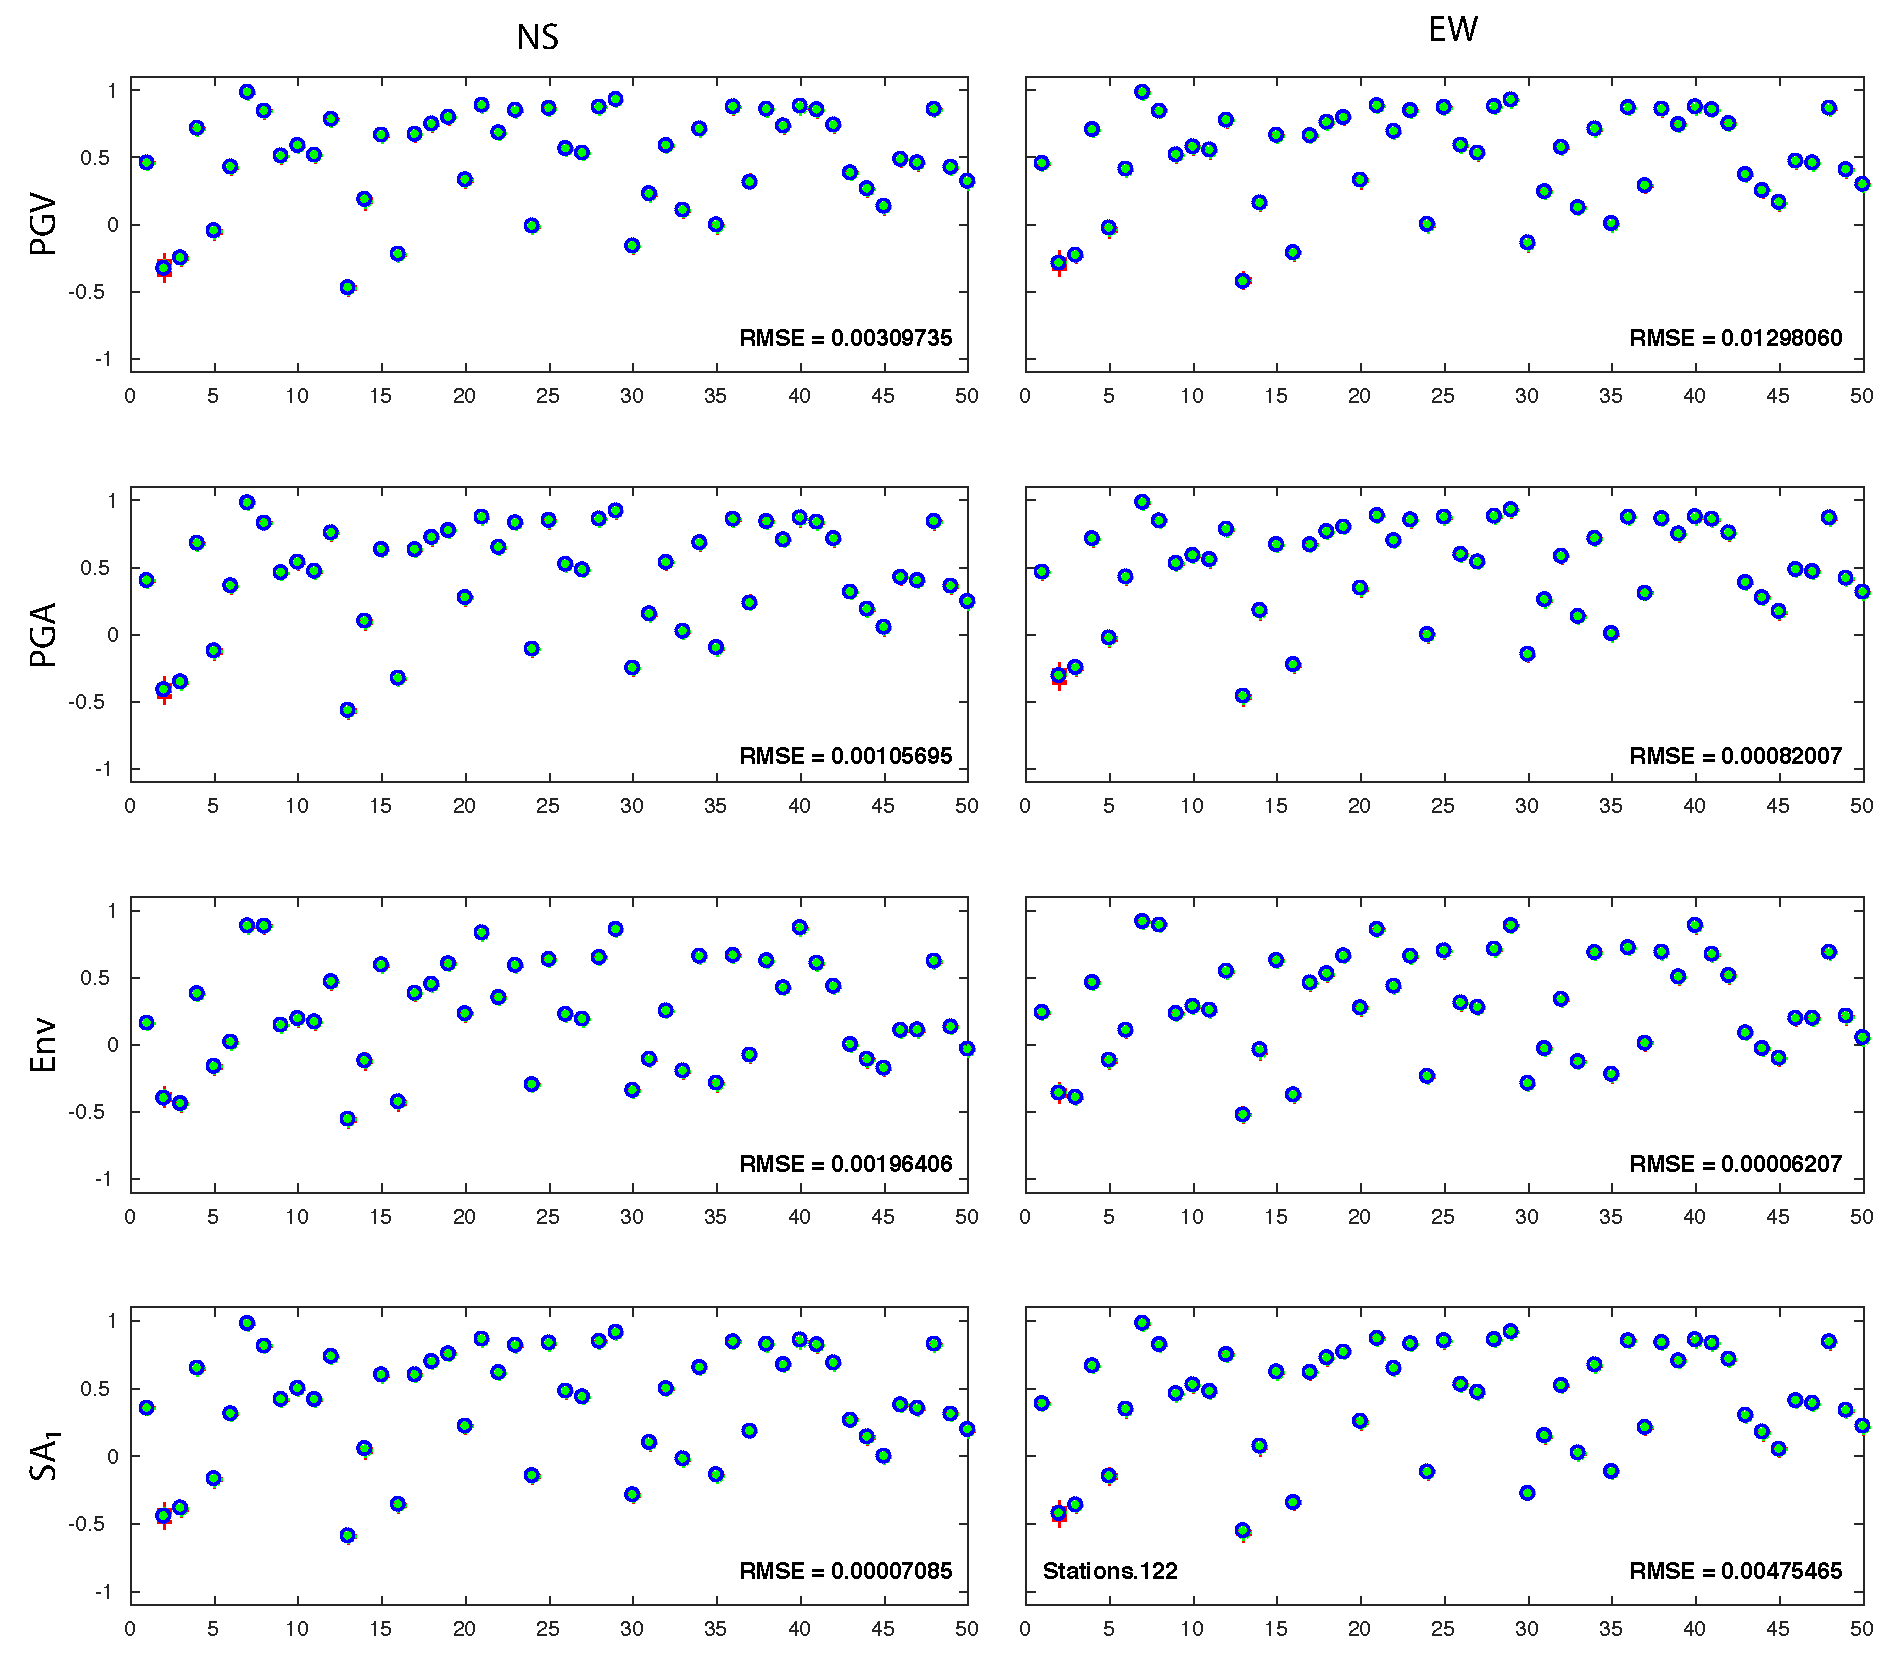
\includegraphics[width=\textwidth]{figures/pdf/Figure_19-st122_het_sim_177.pdf}
    \caption{Accuracy of the results for station number 122 in the heterogenous domain. The station is located in about 42 km from the source (hypo central distance).  }
    \label{fig:ANN_accuracy_stations_122_heterogenous_sim_177}
\end{figure}
 
We follow the steps that we explained at methodology section. We compute the mean of 50 optimized $Q$ values and find the closest $Q$ equation in the training data. We run the optimization process for estimating the new test value which is very close to observation. This process helps us to understand whether the optimization process can find the actual results where we know the input parameters before hand and is very close to the potential field parameters. Those data which pass the following checklist are added to the final Qs-Vs dataset. The criteria is according below:

\begin{itemize}
\item If synthetic solution is converged for a range of shear wave velocity (Standard deviation is an indication of this situation)
\item If the optimizaiotn process successfully locate the input parameters
\end{itemize}

After passing these steps, we generate a dataset and compute another regression analysis to estimate the \qsvs{} relationship that fits the data. As we can see from idealized domains, not all stations and metrics are equally good in extracting all velocity information. This fact also happens in heterogenous domain with fairly complicated source model. Fig.~\ref{fig:used_stations_example} shows four stations that some velocity range of them can pass the defined criteria. 

  \begin{figure}[ht]
    \centering
    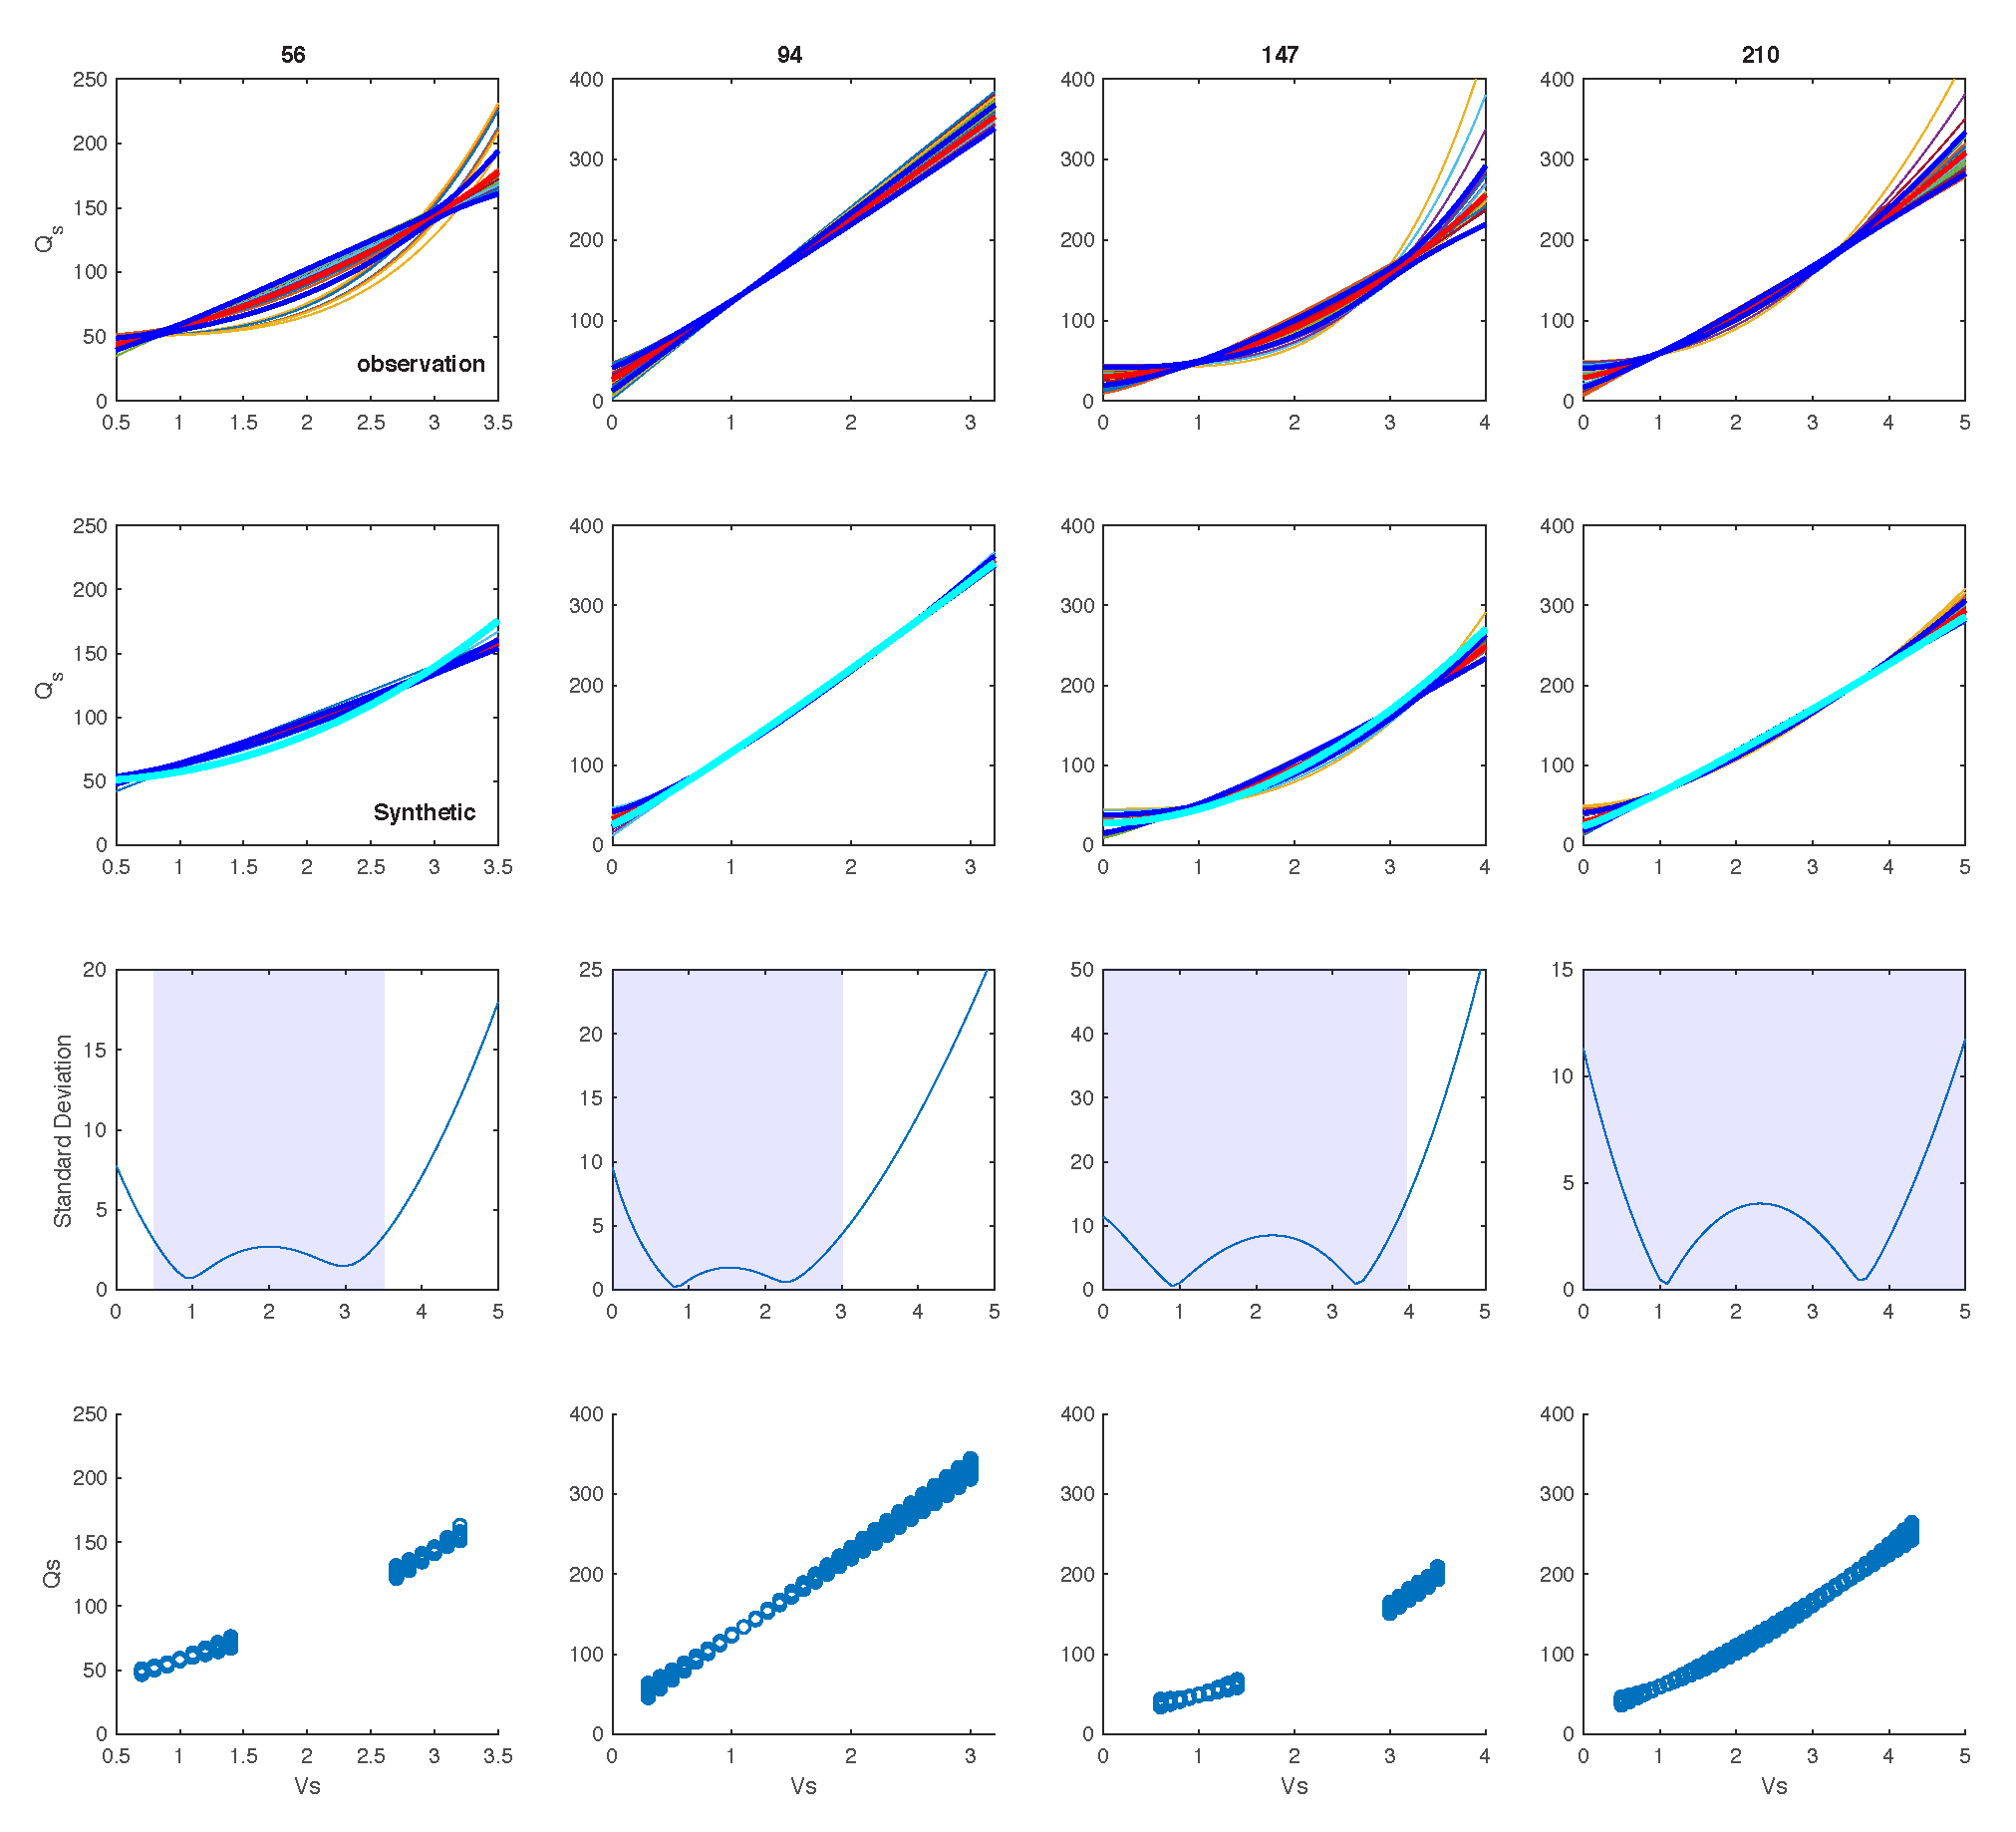
\includegraphics[width=\textwidth]{figures/pdf/Figure_20.pdf}
    \caption{Some of stations in the heterogeneous domain that pass the criteria. The cyan line in synthetic represent the closest available data in training dataset.}
    \label{fig:used_stations_example}
\end{figure}

These four stations are example of stations that part of their shear wave velocity range are used in the final analyses. Each station provides enough information for different range of shear wave velocity. The observation and synthetic are converged at fairly close shear wave velocity ranges for both observation and synthetic. Also in those ranges the algorithm can successfully retrieve the $Q$ value parameters that is used as an input for synthetic target value. The mentioned criteria are met and we can use the results of observation in that range. In order to choose more conservative values for each appropriate shear wave velocity we use only those data that are between $\pm$ standard deviation lines. In all figures these lines are shown using thick blue lines. Similar to the idealized cases, there are stations that cannot pass the defined criteria. Figure.~\ref{fig:unused_stations_example} shows some of these stations. 

  \begin{figure}[ht]
    \centering
    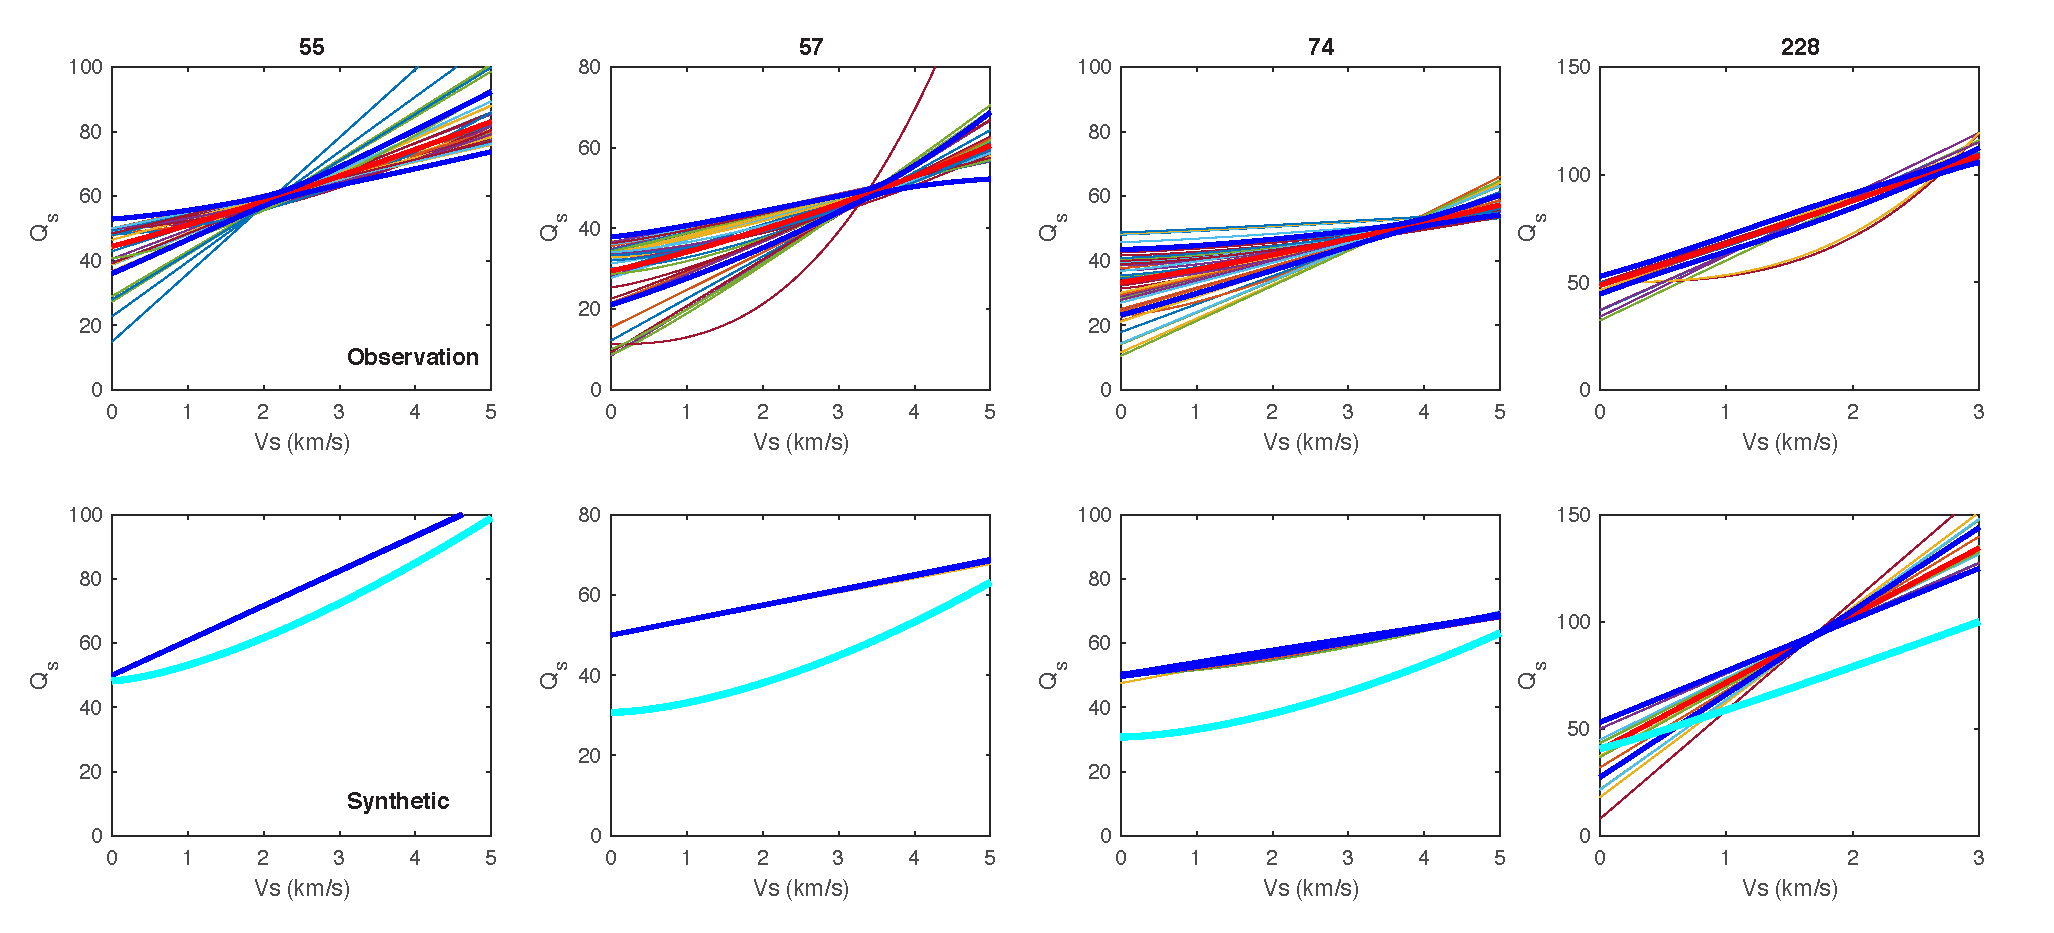
\includegraphics[width=\textwidth]{figures/pdf/Figure_21.pdf}
    \caption{Some of stations in the heterogeneous domain that fails the criteria. }
    \label{fig:unused_stations_example}
\end{figure}

Stations that are represented in Figure.~\ref{fig:unused_stations_example} are not used at the final process. The optimization algorithm provides very converged results at least for three of these stations. However, none of these results are according to the input parameters for target values (dashed green line). This suggests that these stations are not trustable to estimate the observation values. Without the synthetic section of the analyses one arguably can use the converged results of observation. However, the figure shows that the converged $Q$ values are not coincides with initially used $Q$ values. There is a possibility that signal metrics are not conclusive enough to capture the input parameters. The results show that the proposed steps can lead to very accurate and confident parameters. 
The final dataset which we believe is the most appropriate information that we can extract from our dataset in shown in the Fig.~\ref{fig:results_conservative_with_regression} . We use opacity filter and jitter to provide an estimation about the density of points in the figure. In computing the final equation for the Q factor, we ignore data with shear wave velocity less than 350 m/s according to minimum shear wave velocity of the simulations. We use GA optimization to search for the best \qsvs{} relationship that fits dataset.  The final result is $Q_{S}=7.1+60.2 V_{S}^{1.00}$. 


  \begin{figure}[ht]
    \centering
    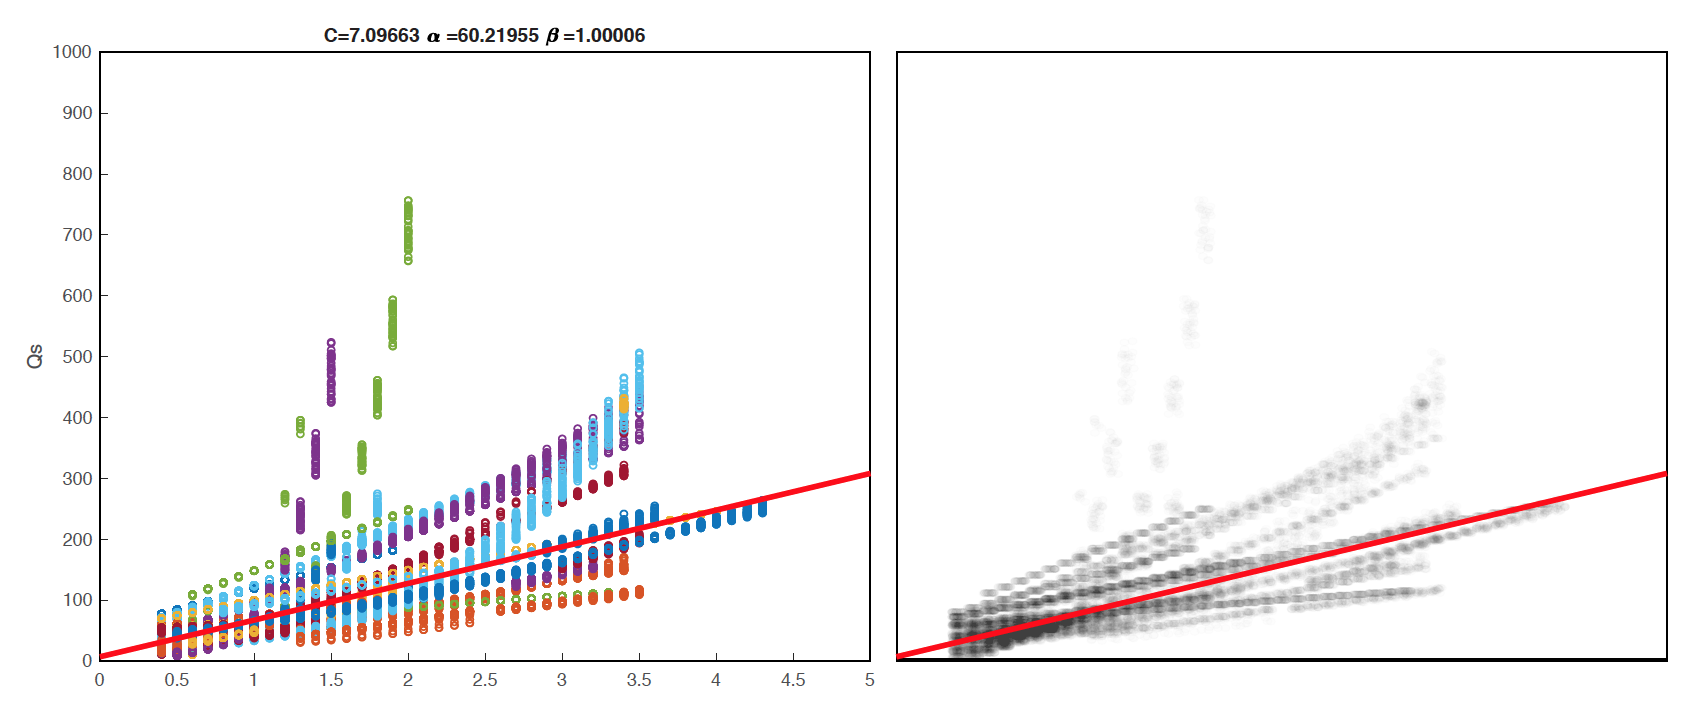
\includegraphics[width=\textwidth]{figures/pdf/Figure_22.png}
    \caption{Scatter data of stations which passed the optimization criteria. Left: Actual data. Different colors represent different stations. Right: Same data with jitter and opacity filter to represent the data density and distribution.}
    \label{fig:results_conservative_with_regression}
\end{figure}





% The proposed method can retrieve two 

% We can argue that there should not be any problem with optimization process.  

%The idea of effective shear wave velocity or average shear wave velocity is not a novel concept. It is used in many different application to estimate the overall shear wave velocity of a soil profile (e.g., see time average method for shear wave velocity in geotechnical engineering applications).  



%\section{Discussion}

We tested the proposed method on 2008 $Mw$ 5.4 ChinoHills earthquake as a heterogeneous medium with real observation.  The proposed equation is shown in Fig.~\ref{fig:Figure_q_models}  along side the comparison of relationships provided in table. ~\ref{tab:QsVstable}. Notice that the majority of the relationships are independent of depth (z). 

 \begin{figure}
    \centering
    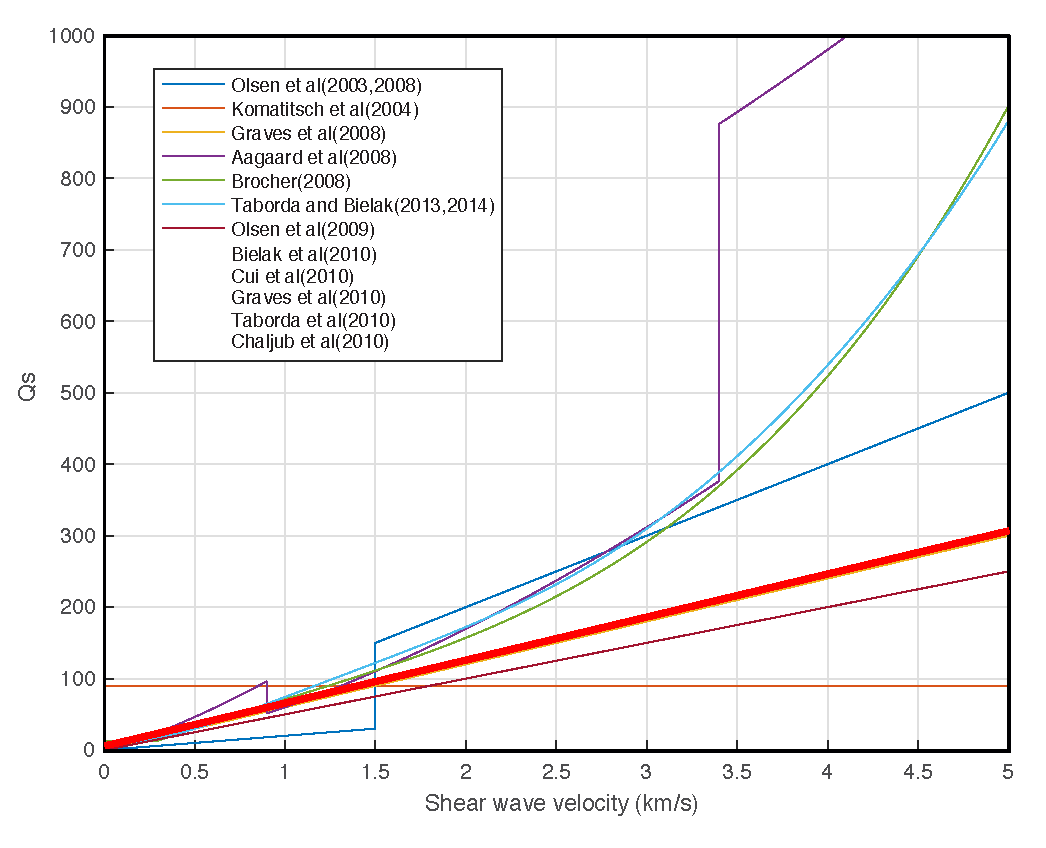
\includegraphics[width=400 px]{figures/pdf/Figure_q_models.pdf}
    \caption{Comparison of Qs rules introduced in table. ~\ref{tab:QsVstable}.}
    \label{fig:Figure_q_models}
\end{figure}

Our proposed relationship---although may not be the definitive one because of limited data used here--- is in agreement with the mean on these values. It is laid between $50Vs$ and $100Vs$ that is commonly used for this region (Lahabra paper, and some other references for 50Vs). Although there is a considerable variation on final dataset shown in Figure.~\ref{fig:results_conservative_with_regression}, the Q equation is not unique for all stations.  Q value is dependent on many other parameters which cause different spatial variation and the end goal is providing a community Q model where all parameters are involved. Variations in QP and QS may be related to porosity, temperature variations, heterogeneity, grain boundary sliding, and lithology. Also, some of the spatial variations in QP and QS appear to be terminated by local fault structure, where on one side of a fault the Q values may be significantly different than on the other \citep{hauksson2006attenuation}.  Moreover, heterogenous domain can cause scattering attention by a redistribution of energy as it is reflected, or converted by small-scale features. These effects may require frequency dependent Q studies \citep{frankel1991mechanisms}.  Also in the near surface sedimentary basin Q is very low \citep{abercrombie1997near}.\\

Therefore, variation of Q values for different stations in a heterogeneous medium are acceptable and predictable. It doubles the importance of the proposed approach where each stations are accurate for different different range of parameters. However, for the physics based ground motion simulation in low frequency, it is a common practice to consider Q only as a function of shear wave velocity. Application of proposed method on simplified, layered and heterogenous medium represents its strong potential and robust behavior towards estimating the most accurate parameters for each station.\\

As we discussed earlier, in several stations peak values of signals in observation (mostly PGV and PGA) are higher than without damping simulation. This can happen due to source parameters (e.g., seismic moment, slip function, ...). Therefore, on other option for better studying the parameters is including source parameters in the ANNs. This can increase the number of training data, however, will give opportunity of involving more stations in the final model.

 




%\section{Conclusion}

We present a customized solution approach to study attenuation models through combining machine learning, ground motion simulation, and optimization process used in physics-based ground motion simulation. We train artificial neural networks and ensemble them though bagging approach as a pseudo-simulator to estimate the signal parameters based on attenuation model inputs. For each station we estimate the approximate Q value through comparing the results with observation and then we understand at which velocity range the stations, model, and optimization process have the potential of providing accurate results. We test the proposed method on homogenous, layered and heterogenous simulation domains. We applied the proposed solution on several stations of 2008 $Mw$ 5.4 ChinoHills earthquake. The results are in agreement with previous studies. We recognize, however, that the proposed equation may not be a definitive one due to use of several stations of one earthquake. In the future follow-up study, it would be ideal to use more signal metrics, more stations and earthquake, as well as include source parameters as an input parameters in pseudo-simulators. The procedural steps laid out here, nonetheless, remain valid.    

In summary, we can say that, in physics based ground motion simulation, artificial neural networks can be easily trained for estimating signal metrics in anelastic domain. These networks can be used in optimization and uncertainty analysis studies. Example of using these networks with optimization algorithm can provide a dominant/effective shear wave velocity for each seismic station. We also show that using only peak ground velocity as a signal metric for estimating Q factor parameters may not be enough and adding other signal parameters improve the results. A combination of machine learning algorithms, optimization process and ground motion simulation can customize the solutions for each individual station and this paper is a successful example of such an application on Q factor parameters studies. 






%\input{acknowledgements}


\bibliographystyle{spbasic}
\bibliography{references_qpaper}


% \section{Introduction}
% \label{sec:introduction}
% Your text comes here. Separate text sections with
% \section{Section title}
% \label{sec:1}
% Text with citations \cite{RefB} and \cite{RefJ}.
% \subsection{Subsection title}
% \label{sec:2}
% as required. Don't forget to give each section
% and subsection a unique label (see Sect.~\ref{sec:1}).
% \paragraph{Paragraph headings} Use paragraph headings as needed.
% \begin{equation}
% a^2+b^2=c^2
% \end{equation}

% % For one-column wide figures use
% \begin{figure}
% % Use the relevant command to insert your figure file.
% % For example, with the graphicx package use
%   \includegraphics{example.eps}
% % figure caption is below the figure
% \caption{Please write your figure caption here}
% \label{fig:1}       % Give a unique label
% \end{figure}
% %
% % For two-column wide figures use
% \begin{figure*}
% % Use the relevant command to insert your figure file.
% % For example, with the graphicx package use
%   \includegraphics[width=0.75\textwidth]{example.eps}
% % figure caption is below the figure
% \caption{Please write your figure caption here}
% \label{fig:2}       % Give a unique label
% \end{figure*}
% %
% % For tables use
% \begin{table}
% % table caption is above the table
% \caption{Please write your table caption here}
% \label{tab:1}       % Give a unique label
% % For LaTeX tables use
% \begin{tabular}{lll}
% \hline\noalign{\smallskip}
% first & second & third  \\
% \noalign{\smallskip}\hline\noalign{\smallskip}
% number & number & number \\
% number & number & number \\
% \noalign{\smallskip}\hline
% \end{tabular}
% \end{table}


%\begin{acknowledgements}
%If you'd like to thank anyone, place your comments here
%and remove the percent signs.
%\end{acknowledgements}

% BibTeX users please use one of
%\bibliographystyle{spbasic}      % basic style, author-year citations
%\bibliographystyle{spmpsci}      % mathematics and physical sciences
%\bibliographystyle{spphys}       % APS-like style for physics
%\bibliography{references}   % name your BibTeX data base


% Non-BibTeX users please use
% \begin{thebibliography}{}
% %
% % and use \bibitem to create references. Consult the Instructions
% % for authors for reference list style.
% %
% \bibitem{RefJ}
% % Format for Journal Reference
% Author, Article title, Journal, Volume, page numbers (year)
% % Format for books
% \bibitem{RefB}
% Author, Book title, page numbers. Publisher, place (year)
% % etc
% \end{thebibliography}

\end{document}

